%&bericht

%%%%%%%%%%%%%%%%%%%%%%%%%%%%%%%%%%%%%%%%%%%%%%%%%%%%%%%%%%%%%%%%%%%%%%%%%%%%%%%
%% Descr:       Vorlage für Berichte der DHBW-Karlsruhe
%% Author:      Prof. Dr. Jürgen Vollmer, juergen.vollmer@dhbw-karlsruhe.de
%% $Id: bericht.tex,v 1.25 2020/03/13 15:07:45 vollmer Exp $
%%  -*- coding: utf-8 -*-
%%%%%%%%%%%%%%%%%%%%%%%%%%%%%%%%%%%%%%%%%%%%%%%%%%%%%%%%%%%%%%%%%%%%%%%%%%%%%%%

\documentclass[
   ngerman          % neue deutsche Rechtschreibung
  ,a4paper          % Papiergrösse
% ,twoside          % Zweiseitiger Druck (rechts/links)
% ,10pt             % Schriftgrösse
  ,11pt
% ,12pt
  ,pdftex
%  ,disable         % Todo-Markierungen auschalten
]{report}

% Bitte die Codierung Ihrer Dateien auswählen:
% \usepackage[latin1]{inputenc}    % Für UNIX mit ISO-LATIN-codierten Dateien
% \usepackage[applemac]{inputenc}  % Für Apple Mac
% \usepackage[ansinew]{inputenc}   % Für Microsoft Windows
\usepackage[utf8]{inputenc}        % UTF-8 codierte Dateien
                                   % Dieses Dokument ist unter Unix erstellt, daher
                                   % wird diese Input-Codierung benutzt.

\usepackage{bericht}

%% ACHTUNG, wenn man eine eigene Formatdatei (bericht.fmt) benutzt, werden Änderungen an bericht.sty
%% erst wirksam, wenn die Format-Datei neu erzeugt wurde!!!
%% Genauer alle Änderungen, die textuell vor der nächsten Zeile ".... endofdump...." stehen
%% werden erst wirksam, wenn die Formatdatei neu erzeugt wurde
\csname endofdump\endcsname

%%%%%%%%%%%%%%%%%%%%%%%%%%%%%%%%%%%%%%%%%%%%%%%%%%%%%%%%%%%%%%%%%%%%%%%%%%%%%%%
%% Angaben zur Arbeit
%%%%%%%%%%%%%%%%%%%%%%%%%%%%%%%%%%%%%%%%%%%%%%%%%%%%%%%%%%%%%%%%%%%%%%%%%%%%%%%

\newcommand{\Autor}{Lukas Hörnle & Marc Gökce}
\newcommand{\MatrikelNummer}{4711}
\newcommand{\Kursbezeichnung}{tinf17b3}

\newcommand{\FirmenName}{Firmenname}
\newcommand{\FirmenStadt}{Stadt}
\newcommand{\FirmenLogoDeckblatt}{\fbox{
\includegraphics[width=3cm]{lion}}}

% Falls es kein Firmenlogo gibt:
%  \newcommand{\FirmenLogoDeckblatt}{}

\newcommand{\BetreuerFirma}{Titel Vorname Nachname}
\newcommand{\BetreuerDHBW}{Titel Vorname Nachname}

%%%%%%%%%%%%%%%%%%%%%%%%%%%%%%%%%%%%%%%%%%%%%%%%%%%%%%%%%%%%%%%%%%%%%%%%%%%%%%%%%%%%%

% Wird auf dem Deckblatt und in der Erklärung benutzt:
\newcommand{\Was}{Studienarbeit}
%\newcommand{\Was}{Projektrarbeit}
%\newcommand{\Was}{Studienarbeit}
%\newcommand{\Was}{Bachleorarbeit}

%%%%%%%%%%%%%%%%%%%%%%%%%%%%%%%%%%%%%%%%%%%%%%%%%%%%%%%%%%%%%%%%%%%%%%%%%%%%%%%%%%%%%

\newcommand{\Titel}{\LaTeX-Vorlage für diverse Ausarbeitungen\\--\\oder so ähnlich}
\newcommand{\AbgabeDatum}{1. April 2090}

\newcommand{\Dauer}{12 Wochen}

% \newcommand{\Abschluss}{Bachelor of Engineering}
\newcommand{\Abschluss}{Bachelor of Science}

\newcommand{\Studiengang}{Informatik / Informationstechnik}
% \newcommand{\Studiengang}{Informatik / Angewandte Informatik}

\hypersetup{%%
  pdfauthor={\Autor},
  pdftitle={\Titel},
  pdfsubject={\Was}
}

%%%%%%%%%%%%%%%%%%%%%%%%%%%%%%%%%%%%%%%%%%%%%%%%%%%%%%%%%%%%%%%%%%%%%%%%%%%%%%%

% Wenn \includeonly{..} benutzt wird, werden nur diese Kaptitel ausgegeben.
\includeonly{
  abk
 ,kapitel1
 ,kapitel2
 ,kapitel3
 ,kapitel4
 ,kapitel5
 ,kapitel6
 ,changelog
}

%%%%%%%%%%%%%%%%%%%%%%%%%%%%%%%%%%%%%%%%%%%%%%%%%%%%%%%%%%%%%%%%%%%%%%%%%%%%%%%

% Benutzt man das "biblatex"-Paket, dann muß das hier stehen:
% siehe auch die mit BIBLATEX markierten Zeilen in bericht.sty
\bibliography{bericht}

\begin{document}

%%%%%%%%%%%%%%%%%%%%%%%%%%%%%%%%%%%%%%%%%%%%%%%%%%%%%%%%%%%%%%%%%%%%%%%%%%%%%%%

\begin{titlepage}
\begin{center}
\vspace*{-2cm}
\FirmenLogoDeckblatt\hfill
\includegraphics[width=4cm]{dhbw-logo}\\[2cm]
{\Huge \Titel}\\[1cm]
{\Huge\scshape \Was}\\[1cm]
{\large für die Prüfung zum}\\[0.5cm]
{\Large \Abschluss}\\[0.5cm]
{\large des Studienganges \Studiengang}\\[0.5cm]
{\large an der}\\[0.5cm]
{\large Dualen Hochschule Baden-Württemberg Karlsruhe}\\[0.5cm]
{\large von}\\[0.5cm]
{\large\bfseries \Autor}\\[1cm]
{\large Abgabedatum \AbgabeDatum}
\vfill
\end{center}
\begin{tabular}{l@{\hspace{2cm}}l}
Bearbeitungszeitraum	         & \Dauer 			\\
Matrikelnummer	                 & \MatrikelNummer		\\
Kurs			         & \Kursbezeichnung		\\
Ausbildungsfirma	         & \FirmenName			\\
			         & \FirmenStadt			\\
Betreuer der Ausbildungsfirma	 & \BetreuerFirma		\\
Gutachter der Studienakademie	 & \BetreuerDHBW		\\
\end{tabular}
\end{titlepage}

%%%%%%%%%%%%%%%%%%%%%%%%%%%%%%%%%%%%%%%%%%%%%%%%%%%%%%%%%%%%%%%%%%%%%%%%%%%%%%%

%%%%%%%%%%%%%%%%%%%%%%%%%%%%%%%%%%%%%%%%%%%%%%%%%%%%%%%%%%%%%%%%%%%%%%%%%%%%%%%
%% Descr:       Vorlage für Berichte der DHBW-Karlsruhe, Erklärung
%% Author:      Prof. Dr. Jürgen Vollmer, vollmer@dhbw-karlsruhe.de
%% $Id: erklaerung.tex,v 1.11 2020/03/13 14:24:42 vollmer Exp $
%% -*- coding: utf-8 -*-
%%%%%%%%%%%%%%%%%%%%%%%%%%%%%%%%%%%%%%%%%%%%%%%%%%%%%%%%%%%%%%%%%%%%%%%%%%%%%%%

% In Bachelorarbeiten muss eine schriftliche Erklärung abgegeben werden.
% Hierin bestätigen die Studierenden, dass die Bachelorarbeit, etc.
% selbständig verfasst und sämtliche Quellen und Hilfsmittel angegeben sind. Diese Erklärung
% bildet das zweite Blatt der Arbeit. Der Text dieser Erklärung muss auf einer separaten Seite
% wie unten angegeben lauten.

\newpage
\thispagestyle{empty}
\begin{framed}
\begin{center}
\Large\bfseries Erklärung
\end{center}
\medskip
\noindent
% siehe §5(3) der \enquote{Studien- und Prüfungsordnung DHBW Technik} vom 29.\,9.\,2017 und Anhang 1.1.13
Ich versichere hiermit, dass ich meine \Was mit dem Thema:
\enquote{\Titel}
selbstständig verfasst und keine anderen als die angegebenen Quellen und Hilfsmittel benutzt habe. Ich versichere zudem, dass die eingereichte elektronische Fassung mit der gedruckten Fassung übereinstimmt.
\vspace{3cm}
\noindent
\underline{\hspace{4cm}}\hfill\underline{\hspace{6cm}}\\
Ort~~~~~Datum\hfill Unterschrift\hspace{4cm}
\end{framed}

\vfill
\emph{Sofern  vom Dualen Partner ein Sperrvermerk gewünscht wird, ist folgende Formulierungzu verwenden:}
\begin{framed}
\begin{center}
\Large\bfseries Sperrvermerk
\end{center}
\medskip
\noindent
Der Inhalt dieser Arbeit darf weder als Ganzes noch in Auszügen Personen
außerhalb des Prüfungsprozesses und des Evaluationsverfahrens zugänglich gemacht
werden, sofern keine anderslautende Genehmigung vom Dualen Partner vorliegt.
\end{framed}

%%%%%%%%%%%%%%%%%%%%%%%%%%%%%%%%%%%%%%%%%%%%%%%%%%%%%%%%%%%%%%%%%%%%%%%%%%%%%%%
\endinput
%%%%%%%%%%%%%%%%%%%%%%%%%%%%%%%%%%%%%%%%%%%%%%%%%%%%%%%%%%%%%%%%%%%%%%%%%%%%%%%


%%%%%%%%%%%%%%%%%%%%%%%%%%%%%%%%%%%%%%%%%%%%%%%%%%%%%%%%%%%%%%%%%%%%%%%%%%%%%%%

\begin{abstract}
Dieses \LaTeX-Dokument kann als Vorlage für einen Praxis- oder Projektbericht, eine Studien- oder
Bachelorarbeit dienen.

Zusammengestellt von Prof.\,Dr.\,Jürgen Vollmer \email{juergen.vollmer@dhbw-karlsruhe.de}\\
\url{https://www.karlsruhe.dhbw.de}. Die jeweils aktuellste Version dieses \LaTeX-Paketes ist immer
auf der \emph{FAQ-Seite} des Studiengangs Informatik zu finden:
\url{https://www.karlsruhe.dhbw.de/inf/studienverlauf-organisatorisches.html} $\to$ \emph{Formulare und Vorlagen}.

\centering Stand \verb+$Date: 2020/03/13 15:07:45 $+
\end{abstract}

\newpage
\tableofcontents           % Inhaltsverzeichnis hier ausgeben

% Jetzt kommt der "eigentliche" Text




\chapter{Einleitung}

\begin{center}
\begin{figure}[h]
    
\includegraphics[width=\textwidth]{img/PIA23645_PaleBlueDotRevisited_1600.jpg}
    \caption{``The Pale Blue Dot'' Feb. 14, 1990, by NASA\footnotemark.}
    \vspace{-6mm}
    \label{fig:my_label}
\end{figure}
\footnotetext{\fullcite{nasa.bluedot}}
\end{center}

''Ein Bild sagt mehr aus als tausend Worte.`` Dieses bekannte Sprichwort drückt aus, wie mächtig Bilder als Kommunikationsmittel sind. 
Bilder beinhalten Informationen, vermitteln Emotionen, erzählen Geschichten und sind ein Fenster in die Vergangenheit. 
Bilder sind in der modernen Gesellschaft omnipräsent und im Alltag digital als auch analog unentbehrlich.
Bilder unterscheiden sich je nach Aufnahme in den verschiedenen Eigenschaften ihrer Speicherung und Darstellung. 
Zwei dieser Eigenschaften sind die Größe und die Auflösung eines Bildes. 
Die Größe eines digitalen Bildes gibt an, wie viele Pixel es enthält, während die Auflösung eines Bildes angibt, wie viele Pixel pro Flächeneinheit vorhanden sind \ac{PPI}.

~

Die Größe und die Auflösung eines Bildes haben Einfluss auf seine Qualität und seinen Speicherplatzbedarf. 
Um ein Bild für einen bestimmten Zweck zu nutzen, muss es häufig in seiner Größe und oder Auflösung verändert werden. 
Der Vorgang zur Veränderung der Größe und Auflösung wird als Bildskalierung bezeichnet\footfullcite{techlib.scaling}\footfullcite{abcdef.scaling} und ist eine grundlegende Operation in der digitalen Bildverarbeitung.
Bildskalierung ist eine grundlegende Methode der Bildverarbeitung. Bildskalierung erlaubt die Änderung der Größe eines digitalen Bildes.
Eine Gute Bildskalierung misst sich an ihren Eigenschaften in den Bereichen Rechenaufwand und Qualitätsverlust. 
Besonders wichtig ist der Qualitätsverlust, wenn man Bilder größer skaliert. 
Ein geeignetes Modell um diesen Prozess zu erklären ist das übertragen einer Zeichnung von einem kleinen Papier auf eine große Leinwand. 
Wird die Zeichnung lediglich unbedacht vergrößert, wird diese unscharf und verliert an Details. 
Das Ziel einer guten Bildskalierung ist es, diesen Effekt zu verhindenr und die Zeichnung größenunabhängig scharf und detailreich darzustellen.

~

Es gibt viele verschiedene Methoden, um die Größe eines Bildes zu ändern. 
Klassische Methoden verwenden Interpolationstechniken, die neue Pixel aus den vorhandenen Pixeln berechnen. 
Diese Methoden sind schnell und stellen einen geringen Rechenaufwand in Kombination mit geringer Komplexität dar. 
Jedoch kommt es mit diesen Algorithmen oft zu Qualitätsverlusten oder der Erzeugung von Artefakten. 
Moderne Anwendungen zur Skalierung von Bildern verwenden Deep-Learning-Techniken wie Convolutional Neural Networks \ac{CNN} oder Generative Adversarial Networks \ac{GAN}, die neue Pixel aus einem trainierten Modell erzeugen. 
Diese neuen Methoden sind komplex und benötigen mehr Rechenaufwand, können allerdings die Qualität des Bildes verbessern oder kreative Effekte erstellen.

\begin{figure}[h!]
    \vspace{8mm}
    \centering
    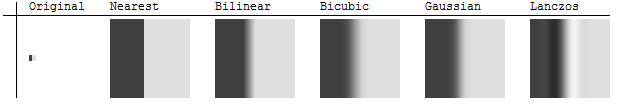
\includegraphics{img/xaR8r.png}
    \caption{Verschiedene Beispiele von upscaling Algorithmen\cite{whuber.lanczos}.}
    \label{fig:my_label}
    \vspace{4mm}
\end{figure}

Die Bildskalierung hat heute viele Anwendungen in verschiedenen Bereichen wie beispielweise Webdesign, Fotografie, Druck oder Videotechnik. 
Es gibt auch in modernen Anwendungen verschiedene Arten von Skalierungsverfahren, die sich in ihrer Funktionsweise und ihrem Ergebnis unterscheiden. 
Diese Arbeit schafft einen Überblick über klassische und moderne Skalierungsverfahren sowie deren ihre Vor- und Nachteile. 
Diese werden anhand von Beispielen inszeniert. 
Zuletzt wird basierend auf der Evaluierung der verschiedenen Verfahren eine Empfehlung für die beste Skalierungsmethode für verschiedene Bildtypen geben. 

~

In dieser Arbeit geht es darum herauszufinden, welche Methode zum Vergrößern oder Verkleinern von Bildern das beste Gleichgewicht aus Komplexität, Rechenaufwand und Ergebnissen liefert. 
Des weiteren werden die Kriterien zur Bewertung von solchen Methoden umschrieben. 
%TODO mit dem Abschnitt bin ich noch nicht happy
Dazu erklären wir zuerst die wichtigsten Konzepte der digitalen Bildverarbeitung und der Skalierung von Bildern und zeigen einige Beispiele für ihre Anwendung. Danach stellen wir die traditionellen Skalierungsmethoden vor und vergleichen ihre Stärken und Schwächen. Dann zeigen wir die neueren Skalierungsmethoden und vergleichen ihre Stärken und Schwächen. Zum Schluss bewerten wir die verschiedenen Methoden mit verschiedenen Maßstäben für die Bildqualität und geben eine Empfehlung für die beste Methode. Wir fassen unsere Ergebnisse zusammen und besprechen ihre Bedeutung und Einschränkungen.
%----------------------
\newpage




\chapter{Grundlagen der Bildverarbeitung und der Skalierung von Bildern}


\section{Einblick in die Bildverarbeitung}
Historie, Entwicklung, aktueller Stand und mögliche Entwicklungen.

\section{Skalierung von Bildern}

\subsection{Arten der Skalierungen: Interpolation und Skalierung}
    Die Interpolation und die Skalierung von Bildern oder Bildbereichen sind wichtige Konzepte der Bildverarbeitung. 
    Das Verfahren der Interpolation ermöglicht es neue Pixelwerte auf Basis vorgegebener Werte zu berechnen.
    Die Skalierung ist eine Anpassung der Bildgröße durch das Ändern der Anzahl von Pixeln oder der Auflösung.
    Im Kontext der Bildverarbeitung wird Interpolation häufig verwendet, um die Größe von Bildern zu ändern, ohne dass dabei die Anzahl der Pixel verändert wird. Dazu werden neue Pixelwerte berechnet, indem vorhandene Pixelwerte interpoliert werden. 
    Die Wahl der Interpolationsmethode hat einen großen Einfluss auf die Qualität des interpolierten Bildes. 
    In der Bildverarbeitung gibt es verschiedene Interpolationsmethoden, wie z.B. Nearest-Neighbor-Interpolation, Bilineare Interpolation oder Bikubische Interpolation.
    Skalierung hingegen verändert die Größe eines Bildes, indem die Anzahl der Pixel oder die Auflösung verändert wird. 
    Im Gegensatz zur Interpolation wird die Anzahl der Pixel bei der Skalierung verändert, um das Bild kleiner oder größer zu machen. 
    Auch hier hat die Wahl der Skalierungsmethode einen großen Einfluss auf die Qualität des resultierenden Bildes.

\subsection{Bildformate}
    Bilder können allgemein als zweidimensionaler Array dargestellt werden.
    Historisch gesehen gab es jedoch viele unterschiedliche Formate für Bilder. 
    Zunächst erschufen unterschiedliche Softwareentwickler im Bereich der Bildverarbeitung häufig ihre eigenen Formate.\footfullcite{burger2009digitale}
    Einheitliche Standards, wie sie heute im Einsatz sind, etablierten sich erst später.
    Ein Vorreiter der modernen Bildformate ist das "Portable Network Graphics Format"\footfullcite{boutellpng}, das 1985 in den USA vorgestellt wurde. 
    Moderne Dateiformate zur Speicherung von Bildern werden anhand der Art des Bildes sowie der Kriterien Speicherbedarf und Kompression, Kompatibilität und ihrem Anwendungsbereich bewertet. 
    \footfullcite{burger2009digitale}
    
    \subsubsection{Portable Network Graphics Format}
        Portable Network Graphics Format \ac{PNG} setzt einen besonderen Fokus auf eine geringe Komplexität und eine einfache Implementierung des Standards. 
        Der Standard kann frei von jedem genutzt werden.
        Des weiteren profitiert das Format von verlustfreier Kompression. \footfullcite{boutell1997png}
        PNG unterstützt Vollfarbbilder, Grauwertbilder sowie Indexbilder. \footfullcite{burger2015digitale}
        Der PNG-Algorithmus komprimiert Bilder, indem er mehrere Techniken, einschließlich Filterung und Huffman-Codierung anwendet. 
        Zunächst wird das Bild in Blöcke von 16 x 16 Pixeln aufgeteilt und dann wird auf jedem Block ein Filter angewendet, um Redundanzen zu entfernen. 
        Anschließend wird das Ergebnis der Filterung Huffman-codiert, um eine effiziente Darstellung der Daten zu erreichen.
        Characteristisch für PNG-Dateien ist auch die Möglichkeit, transparente Flächen einzubauen. 
        Der Standard verwendet eine spezielle Methode, um Transparenz darzustellen. 
        Diese wird als Alpha-Kanal bezeichnet und ermöglicht es, transparente sowie halbtransparente Bilder zu erstellen.
        Die kompekte Komprimmierung des PNG-Formats hat dafür gesorgt, dass der Standard im Internet eine hohe Beliebtheit genießt. 
        \footfullcite{^w3c_png}
    
    \subsubsection{JPG-Format}
        \ac{JPG}
        %TODO und Acronym für JPG
        Hier noch text bittö.
        
    
    \subsubsection{Scalable Vector Graphics}
        \begin{quote}
            The main idea motivating \ac{SVG} was simple: to create a generic document-oriented solution  for graphics that can be adapted to modern media
            \grqq{}~\footfullcite{book:729077}
        \end{quote}
        %Evaluation und Implementierung eines Bildverarbeitungsverfahrens zur Füllstandsmessung
        Scalable Vector Graphics (SVG) steht für ein Format, das Vektorgrafiken basierend auf \ac{XML} darstellt.
        Im Gegensatz zu Rastergrafiken, wie z.B. PNG, die aus Pixeln bestehen und bei Vergrößerung an Schärfe verlieren, sind Vektorgrafiken vektorbasiert und behalten ihre Qualität bei beliebiger Skalierung. 
        Der Standard ermöglicht eine besonders effiziente Speicherung von Bildern.
        SVG ist außerdem ein offenes Format und unterstützt Interaktivität, Animation und Skripting.\footfullcite{quint2003scalable} 
        Da SVG auf XML basiert, kann es auch mit anderen Webtechnologien wie HTML, \ac{CSS} und JavaScript integriert werden.\footfullcite{mdn_svg} 
        
    \subsubsection{Weitere Standards}
        %TODO MEHR TEXT!!!! 
        \begin{description}
            \item[\ac{GIF}]~\\
                Ein Format für animierte Rastergrafiken mit einer begrenzten Farbpalette von 256 Farben. 
                Es verwendet eine verlustfreie Kompression, die aber nicht sehr effizient ist. 
                Es ist geeignet für einfache Animationen und Grafiken mit wenigen Farben.
            \item[\ac{TIFF}]~\\
                Ein Format für hochauflösende Rastergrafiken ohne Kompression oder mit verlustfreier Kompression.
                Es wird oft im Druckbereich verwendet, da es viele Optionen für Farbmanagement und Metadaten bietet.
                Es ist aber nicht sehr kompatibel mit Webbrowsern \\
            \item[\ac{PSD}]~\\
                Ein Format für Photoshop-Dokumente, das alle Ebenen, Masken, Effekte und andere Informationen speichert.
                Es ermöglicht eine umfangreiche Bearbeitung von Rastergrafiken, ist aber nur mit Photoshop kompatibel.\\
            \item[\ac{BMP}]~\\
                Ein Format für unkomprimierte Rastergrafiken mit hoher Qualität.
                Es wird selten verwendet, da es sehr große Dateien erzeugt und keine Transparenz oder andere Funktionen unterstützt. \\
            \item[\ac{EPS}]~\\
                Ein Format für vektorbasierte Grafiken, das Kurven, Texte und andere Elemente speichert.
                Es kann skaliert werden ohne Qualitätsverlust und wird oft im Druckbereich verwendet.
                Es ist aber nicht sehr kompatibel mit Webbrowsern oder anderen Programmen. \\
        \end{description}
        Weiterhin gibt es unzählige Standards um Grafiken darzustellen. Diese übersteigen jedoch den Umfang dieser Arbeit.
        \footfullcite{prepressure_file_formats}\footfullcite{ionos_file_formats}\footfullcite{rabbani2002overview}\footfullcite{marcellin2000overview}\footfullcite{britannica_jpeg}\footfullcite{elsevier_artwork}
\subsection{Wichtige Aspekte der Skalierung}
    \subsubsection{Segmentierung}
    
        Die Segmentierung von Bildern ist ein wichtiges Verfahren der Bildverarbeitung, da es ermöglicht, ein Bild in sinnvolle Regionen zu unterteilen. 
        Hierbei können verschiedene Verfahren, wie Schwellenwert- oder Clustering-Methoden eingesetzt werden. 
        Die Genauigkeit der Segmentierung hängt dabei maßgeblich von der Komplexität des Bildes und der gewählten Methode ab.
        Eine erfolgreiche Segmentierung kann für viele Anwendungen von Nutzen sein.
        Die automatischen Erkennung von Gesichtern oder die Identifizierung von Verkehrszeichen auf Straßenbildern sind die populärsten Beispiele.
        Jedoch ist es oft schwer genaue Grenzen zwischen Objekten in Bildern mit komplexen Strukturen zu erkennen.
    
    \subsubsection{Klassifizierung}
    
        Die Klassifizierung von Bildinhalten ist ein weiterer wichtiger Aspekt der Bildverarbeitung.
        Hierbei werden Bilder in automatisch bestimmte Kategorien eingeteilt. 
        Beispielanwendungen inkludieren das Erkennen von Tierarten auf Naturfotos oder das Identifizieren von Gesichtern auf Fotos. 
        Hierfür können verschiedene Techniken verwendet werden. Beispiele sind Deep Learning oder Entscheidungsbaum-Algorithmen.
        Eine erfolgreiche Klassifizierung kann für viele Anwendungen genutzt werden, wie zum Beispiel zur Automatisierung von Aufgaben oder im maschinellen Lernen. 
        Die Geneauigkeit einer Klassifizierung wird von Faktoren, wie zum Beispiel von der Qualität der Trainingsdaten oder der Komplexität der verwendeten Klassifikationsmethode beeinflusst.
    
    \subsubsection{Objekterkennung und -verfolgung}
    
        Die Objekterkennung und -verfolgung ist ein wichtiger Aspekt der Bildverarbeitung, der oft in Anwendungen wie der Überwachung und Robotik genutzt wird. 
        Hier geht es darum, Objekte in Bildern oder Videos zu erkennen und ihre Bewegungen zu verfolgen. 
        Es können verschiedene Techniken eingesetzt werden, wie zum Beispiel Hintergrundsubtraktion oder optische Flussberechnung.
        Eine erfolgreiche Objekterkennung und -verfolgung kann für viele Anwendungen genutzt werden, wie zum Beispiel in der Videoüberwachung oder bei der Steuerung von autonomen Fahrzeugen. 
        Allerdings gibt es auch Herausforderungen bei der Objekterkennung und -verfolgung, wie zum Beispiel die Bewältigung von Hintergrundrauschen oder die Verfolgung von Objekten bei hoher Geschwindigkeit.
    
    \subsubsection{3D-Bildverarbeitung}
        In der 3D-Bildverarbeitung werden dreidimensionale Bilder und Modelle analysiert und verarbeitet.
        Die Anwendungsfelder dieser Technologien reichen von medizinischen Umgebungen bis hin zur industriellen Fertigung.
        In bildgebenden medizinischen verfahren werden 3D-Bilder für die Diagnose von Krankheiten und Verletzungen verwendet. 
        In der industriellen Fertigung werden 3D-Modelle für die Qualitätssicherung und die Fehlererkennung verwendet.
    
    \subsubsection{Bildkompression}
        Da Bilder in der Regel große Datenmengen erzeugen, die für die Übertragung und Speicherung unpraktisch sind, benötigt es oft eine Bildkompression. 
        Durch Kompressionstechniken wie z.B. die JPEG-Kompression kann die Größe von Bildern erheblich reduziert werden ohne dabei große QUalitätsverluste zu erleiden.
    
\section{Echtzeitverarbeitung von Bildern}

    Die Echtzeitverarbeitung von Bildern stellt eine Herausforderung in der Bildverarbeitung dar, da eine sehr schnelle Verarbeitung notwendig ist, um zeitkritische Anwendungen wie z.B. autonomes Fahren oder Augmented Reality zu realisieren.
    Bei diesen Aufgaben müssen Bilder in Echtzeit erfasst, verarbeitet und angezeigt werden, um eine reibungslose Funktionalität zu gewährleisten.
    Die Echtzeitverarbeitung von Bildern erfordert in der Regel eine hohe Rechenleistung, um die Daten schnell genug zu verarbeiten.
    Hierbei kommen spezielle Algorithmen zum Einsatz, die für eine effiziente Verarbeitung sorgen.
    Eine weitere Herausforderung bei der Echtzeitverarbeitung von Bildern ist die Echtzeit-Kommunikation zwischen den verschiedenen Komponenten des Systems. 
    Hierbei müssen Daten schnell und zuverlässig ausgetauscht werden, um Verzögerungen zu vermeiden. 
    Hierfür kommen oft spezielle Systeme zum Einsatz, die für eine schnelle Übertragung und parallele Verarbeitung von Daten optimiert sind.
    \footfullcite{oehlrich1992transputersystem}
\section{Anwendungen von Skalierungsmethoden}
    % help
    Die Anwendung von Skalierungsmethoden bietet eine Vielzahl ungewöhnlicher, aber äußerst nützlicher Anwendungen in verschiedenen Sektoren.
    In der Landwirtschaft können diese Methoden dazu beitragen, die Gesundheit von Pflanzen zu überwachen und den Einsatz von Pestiziden zu optimieren.
    Durch die Analyse von Pflanzenbildern können frühzeitig Krankheiten erkannt und gezielte Maßnahmen ergriffen werden, um Ernteausfälle zu minimieren.
    In der Archäologie ermöglichen Skalierungsmethoden die digitale Rekonstruktion verwitterter oder beschädigter Artefakte.
    Dies eröffnet Forschern neue Einblicke in die Geschichte vergangener Zivilisationen und ermöglicht die Erstellung interaktiver virtueller Museen.
    In der Modeindustrie ermöglichen Skalierungsmethoden das virtuelle Anprobieren von Kleidung, was den Kunden die Möglichkeit gibt, Passform und Aussehen der Kleidungsstücke im Voraus zu überprüfen und das Online-Shopping-Erlebnis zu verbessern.
    Durch die Integration von Bildverarbeitung und Augmented Reality entsteht eine innovative und interaktive Shopping-Erfahrung.
    Insgesamt bieten Skalierungsmethoden in diesen verschiedenen Sektoren ungewöhnliche Anwendungen, die zu Effizienzsteigerungen, Erkenntnisgewinnen und verbesserten Kundenerfahrungen führen.

\chapter{Klassische Skalierungsmethoden}

    \section{Pixel-Verdopplung}

        \begin{figure}[h]
            \centering
            
\includegraphics[width=0.6\textwidth]{img/so_sieht_pixel_verdopplung_aus.jpg}
            \caption{Beispielhafte Darstellung einer Skalierung durch PixelVerdopplung}
            \label{fig:beispielhafte_darstellung_einer_skalierung_durch_pixelverdopplung}
        \end{figure}

        Die Pixel-Verdopplung vergrößert das Bild, indem jeder Pixel dupliziert wird.
        Diese Methode kann schnell und einfach umgesetzt werden, indem jeder Pixelwert einfach auf den Nachbarpixel übertragen wird.
        Wenn Bilder mit dieser Methode stark vergrößert werden, ergeben sich oft pixelige und unscharfe Ausgaben, da die Details nicht wirklich vorhanden sind, sondern nur durch die Duplizierung von Pixeln aufgefüllt werden. 
        Aus diesem Grund wird Pixel-Verdopplung oft als eine minderwertige Skalierungsmethode betrachtet und findet in professionellen Anwendungen selten Gebrauch.~\footfullcite{WANG1983363}


    \newpage
    Eine beispielhafte Implementierung in Python sieht folgendermaßen aus:
    
    \begin{lstlisting}[caption={Python-Klasse zur Pixelverdopplung und Bildmanipulation: Implementierung des Algorithmus mit der Pillow-Bibliothek und Erklärung des Codes von PixelVerdopplung: \url{https://github.com/studienarbeit-cnn-dhbwka-2022/Code/blob/main/backend/skalierungsmethoden/pixel_verdopplung.py}.}]
    class PixelVerdopplung(Image):
        def __init__(self, path):
            extend = "p2"
            super().__init__(path, extend)
        
        def manipulate(self, new_size):
            super().manipulate(new_size)
        
            for y in range(self.new_height):
                for x in range(self.new_width):
                    x_old = int(x / (self.new_width / self.width))
                    y_old = int(y / (self.new_height / self.height))
        
                    # Check that x_old and y_old are within bounds of original image
                    if x_old >= self.width:
                        x_old = self.width - 1
                    if y_old >= self.height:
                        y_old = self.height - 1
        
                    old_pixel = self.img.getpixel((x_old, y_old))
                    self.newImg.putpixel((x, y), old_pixel)
        
            return self.save()
    \end{lstlisting}
        
        Die vorliegende Implementierung in Python beschreibt die Realisierung der Pixelverdopplungsklasse, welche in der Lage ist, ein größeres Bild zu erzeugen, indem die leeren Pixel mit demselben Pixelwert wie der nächste Nachbarpixel befüllt werden.
        Der Code ist darauf ausgelegt, eine einfache Möglichkeit bereitzustellen, um ein Bild auf eine höhere Auflösung zu skalieren, wodurch fehlende Details ausgeglichen werden können.
        Dabei wird eine lineare Interpolation auf der Basis der Nachbarpixel durchgeführt, um das neue Bild zu generieren.
        Die Klasse "PixelVerdopplung" erbt von der Klasse "Image" und besitzt einen Konstruktor, der den Pfad zum Bild und die Erweiterung "p2" als Argumente erhält. 
        Die Methode "manipulate" ist dafür zuständig, das Bild auf die gewünschte Größe zu skalieren und zu manipulieren.
        Innerhalb der Methode werden Schleifen durchlaufen, um jeden neuen Pixel im manipulierten Bild zu generieren. 
        Die Koordinaten des jeweiligen alten Pixels werden durch Division der neuen Koordinaten durch die Skalierungsfaktoren berechnet und auf den nächstgelegenen Integer gerundet.
        Um sicherzustellen, dass die berechneten Koordinaten innerhalb der Grenzen des ursprünglichen Bildes liegen, werden sie in einem nächsten Schritt auf den maximalen Index des Bildes zurückgesetzt, falls sie außerhalb liegen sollten. 
        Anschließend wird der Pixelwert des entsprechenden alten Pixels abgerufen und als neuer Pixel an der berechneten Stelle im neuen Bild platziert.
        Die Implementierung dieses Algorithmus stellt eine einfache Möglichkeit dar, um ein Bild auf eine höhere Auflösung zu skalieren, wodurch ein besseres visuelles Ergebnis erzielt werden kann. 
        Dabei ist darauf zu achten, dass die lineare Interpolation eine höhere Laufzeit und Speicheranforderungen aufweist als andere Interpolationsmethoden.
        
    \section{Nearest-Neighbor-Interpolation}
        Die Nearest-Neighbor-Interpolation ist eine weitere Methode zur Skalierung von Bildern. 
        Es wird für jedes Pixel im Ausgabebild der am nächsten liegende Pixel im Eingabebild ausgewählt und der Farbwert des ausgewählten Pixels wird als Farbwert des entsprechenden Pixels im Ausgabebild verwendet.
        Die Verwendung von Nearest-Neighbor-Interpolation ist einfach und schnell zu implementieren. 
        Aufgrund ihrer geringen Komplexität ist sie daher sehr beliebt. 
        Die Methode eignet sich besonders gut für die Vergrößerung von Bildern mit großen, einheitlichen Bereichen oder harten Kanten. 
        

        \begin{acronym}
          \acro{NNI}{Nearest Neighbor Interpolation}
        \end{acronym}
        \begin{lstlisting}
        import numpy as np
        import cv2
        
        def nearest_neighbor_interpolation(image, scale_factor):
            new_size = (int(image.shape[1] * scale_factor), int(image.shape[0] * scale_factor))
            
            scaled_image = np.zeros(new_size + (image.shape[2],), dtype=np.uint8)
            for i in range(new_size[0]):
                for j in range(new_size[1]):
                    x = int(i / scale_factor)
                    y = int(j / scale_factor)
                    scaled_image[j, i] = image[y, x]
            
            return scaled_image
        
        
        image = cv2.imread('example_image.jpg')
        scaled_image = nearest_neighbor_interpolation(image, 2)
        cv2.imshow(image)
        cv2.imshow(scaled_image)
        \end{lstlisting}\footfullcite{jiang2015quantum}
        %TODO @Marc kannst du mir ne Schöne Grafik machen, wo du diesen Code kurz über unser Beispielbild laufen lässt und wir so nen rechts/links Vergleich haben?

        Bei der Verkleinerung von Bildern erleiden diese jedoch oft einen Qualitätsverlust.
        Hier kommt es zu Unschärfe und Blockbildung.
        Dieser Effekt verstärkt sich, wenn das Verhältniss zwischen Quellbild und Audgabebild kein Vielfaches ist.

    \section{Bilineare Interpolation}
    
    % Interpolation cool weil, schnell und ergebniss recht schön.

    % Bilinear ist well aus 2 pixel linear interpoliert wird. (Bild farbig)
    % Die Distanz wir linear berechnet aus den 4 nachbar pixel (Graph 2 punkte)
    % wird fast überall genutzt (citation und quelle angeben)
    
    % Vorteile: Schnell und kompilizert zu programmieren, sieht nicht beschissen aus und kann immer angewendet werden
    % Nachteile: Sieht nicht perfekt aus (Siehe Bicubic oder lanzeros) - ist bei extremen skalierungen nicht super

        Die bilineare Interpolation ist eine weit verbreitete Methode zur Skalierung von Bildern.
        Sie basiert auf dem Konzept der linearen Interpolation und wird häufig in Grafikanwendungen und Bildverarbeitungsalgorithmen eingesetzt.
        Bei der bilinearen Interpolation werden zwei Pixelwerte linear interpoliert, um den Wert eines Zwischenpunkts zu berechnen.
        Dieser Ansatz führt zu einer relativ schnellen Berechnung und liefert ästhetisch ansprechende Ergebnisse.

        \begin{figure}[h]
            \centering
            
\includegraphics[width=0.5\textwidth]{img/so_sieht_bilineare_verdopplung_aus}
            \caption{So sieht bilineare Verdopplung aus.}
            \label{fig:so_sieht_bilineare_verdopplung_aus}
        \end{figure}

        Der Prozess der bilinearen Interpolation bezieht sich auf die Berechnung der Distanz zwischen dem zu interpolierenden Punkt und den umliegenden vier Pixeln.
        Diese Distanz wird linear verwendet, um gewichtete Durchschnittswerte der umgebenden Pixel zu erzeugen.
        Dieser Ansatz ermöglicht eine glattere Darstellung von Zwischenwerten im Vergleich zu einfacheren Interpolationsmethoden wie der nächsten Nachbar-Interpolation.


        \begin{figure}[h]
            \centering
            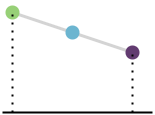
\includegraphics[width=0.5\textwidth]{img/pixel_verdopplung_graph.png}
            \caption{Graph über bilineare Skalierung.}
            \label{fig:graph_uber_bilineare_skalierung}
        \end{figure}

        Die bilineare Interpolation wird aufgrund ihrer Einfachheit und Effizienz häufig eingesetzt.
        Sie ist schnell zu implementieren und kann auf unterschiedliche Bildgrößen angewendet werden.
        Viele Bildbearbeitungssoftware und Grafikbibliotheken nutzen bilineare Interpolation als Standardmethode für die Skalierung von Bildern.
        Dennoch hat die bilineare Interpolation einige Nachteile, insbesondere bei extremen Skalierungen.
        Bei sehr großen oder kleinen Skalierungsfaktoren können Artefakte auftreten, die zu einer verminderten Bildqualität führen.
        In solchen Fällen können fortgeschrittenere Interpolationsverfahren wie Bicubic oder Lanczos eine bessere Wahl sein.


    \begin{figure}[h]
        \centering
        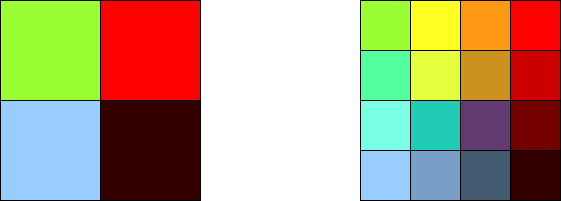
\includegraphics[width=0.5\textwidth]{img/pixel_verdopplung.png}
        \caption{Beispielgrafik zur Pixelverdopplung.}
        \label{fig:beispielgrafik_zur_pixelverdopplung}
    \end{figure}
    
    
    \begin{lstlisting}
    for y in range(self.new_height):
        for x in range(self.new_width):
            x_old = x / (self.new_width / self.width)
            y_old = y / (self.new_height / self.height)
    
            # Find the surrounding pixels
            x1 = int(x_old)
            x2 = min(x1 + 1, self.width - 1)
            y1 = int(y_old)
            y2 = min(y1 + 1, self.height - 1)
    
            # Check if x2 and y2 are out of bounds, if they are substract one
            if x2 == self.width - 1:
                x2 = x1
                x1 -= 1
            if y2 == self.height - 1:
                y2 = y1
                y1 -= 1
    
            # Find the weights
            w1 = (x2 - x_old) * (y2 - y_old)
            w2 = (x_old - x1) * (y2 - y_old)
            w3 = (x2 - x_old) * (y_old - y1)
            w4 = (x_old - x1) * (y_old - y1)
    
            # Get the pixel values of the surrounding pixels
            p1 = self.img.getpixel((x1, y1))
            p2 = self.img.getpixel((x2, y1))
            p3 = self.img.getpixel((x1, y2))
            p4 = self.img.getpixel((x2, y2))
    
            # Interpolate the pixel value
            new_pixel = (
                int(w1 * p1[0] + w2 * p2[0] + w3 * p3[0] + w4 * p4[0]),
                int(w1 * p1[1] + w2 * p2[1] + w3 * p3[1] + w4 * p4[1]),
                int(w1 * p1[2] + w2 * p2[2] + w3 * p3[2] + w4 * p4[2])
            )
            self.newImg.putpixel((x, y), new_pixel)
    \end{lstlisting}\footfullcite{1409828}
    
\section{Bikubische Interpolation}

\subsection{Mathematische Grundlagen}


% Erläuterung der mathematischen Grundlagen der bikubischen Interpolation, einschließlich der Verwendung von kubischen Polynomen und der Stichprobentheorie.
% Herleitung der bikubischen Interpolationsformel und der Eigenschaften der resultierenden Funktion.
% Diskussion der Vor- und Nachteile der Verwendung kubischer Funktionen für die Interpolation im Vergleich zu anderen Funktionstypen.
% Überblick über die Rolle der Fourier-Analyse und der Fourier-Transformationen bei der Bildinterpolation und wie sich dies auf die bikubische Interpolation bezieht.
    
Die bikubische Interpolation ist ein mathematisches Verfahren zur Schätzung der Werte einer kontinuierlichen Funktion an einer gegebenen Stelle, indem eine Funktion mit kubischen Polynomen verwendet wird, die durch benachbarte Funktionswerte verläuft.
Dabei wird das umliegende Gebiet untersucht und die Werte werden basierend auf der Stichprobentheorie geschätzt.

Die bikubische Interpolationsformel ist eine Erweiterung der Bilinearinterpolation auf vier umliegende Pixel und verwendet eine Funktion, die durch benachbarte Funktionswerte verläuft.
Die resultierende Funktion ist stetig differenzierbar und besitzt glatte partielle Ableitungen.

\begin{figure}[h]
    \centering
    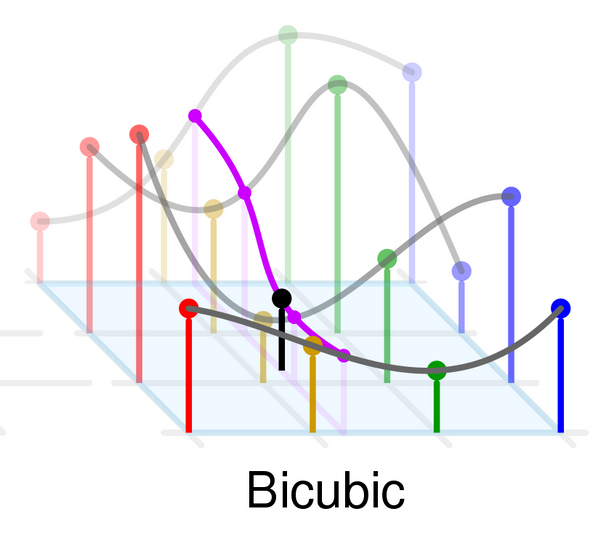
\includegraphics[width=0.5\textwidth]{img/bicubic_graph}
    \caption{Bikubische Interpolation}
    \label{fig:bicubic_interpolation}
\end{figure}

Im Vergleich zu anderen Interpolationsverfahren wie der bilinearen Interpolation und der Lanczos-Interpolation hat die bikubische Interpolation den Vorteil, dass sie eine höhere Genauigkeit bei der Schätzung von Pixelwerten bietet.
Ein Nachteil ist jedoch, dass sie im Allgemeinen höhere Rechenaufwendungen erfordert.

Die Fourier-Analyse und die Fourier-Transformationen spielen eine wichtige Rolle bei der Bildinterpolation, da sie es ermöglichen, die Funktion in den Frequenzraum zu transformieren und damit eine effektivere Interpolation zu erreichen.

\subsection{Algorithmische Implementierung}


% Überblick über die algorithmischen Schritte bei der bikubischen Interpolation, einschließlich der Auswahl der umgebenden Pixel und der Gewichte sowie der Berechnung der neuen Pixelwerte.
% Diskussion von Techniken zur Optimierung der Leistung der bikubischen Interpolation, wie z. B. die Vorberechnung von Lookup-Tabellen, Parallelisierung und Speicherverwaltung.
% Untersuchung von Grenzfällen und Randbedingungen, die bei der bikubischen Interpolation auftreten können, und wie diese effektiv behandelt werden können.
% Vergleich der algorithmischen Implementierung der bikubischen Interpolation mit anderen Interpolationsverfahren, wie z.B. der bilinearen Interpolation und der Lanczos-Interpolation.

    
Die bikubische Interpolation erfolgt durch die Auswahl von umgebenden Pixeln und deren Gewichte sowie der Berechnung der neuen Pixelwerte.

Sie verwendet eine 4x4-Matrix umliegender Pixel, um den Wert an einem bestimmten Punkt zu berechnen.
Die Formel zur Berechnung lautet:

Die Koeffizienten $a_{ij}$ werden basierend auf den umliegenden Pixelwerten und ihren Ableitungen berechnet.
Dieses Verfahren ermöglicht eine glatte Interpolation zwischen den Pixeln und hinterlasst wenige scharfe Kanten.

\begin{equation}
    f(x,y) = \sum_{i=0}^{3}\sum_{j=0}^{3}a_{i,j}*x^{i}*y^{j}
\end{equation}

Eine Möglichkeit zur Optimierung der Leistung besteht darin, Lookup-Tabellen vorzubereiten, Parallelisierungstechniken zu verwenden und die Speicherverwaltung zu optimieren.
Grenzfälle und Randbedingungen können bei der bikubischen Interpolation auftreten und müssen effektiv behandelt werden.
Die algorithmische Implementierung der bikubischen Interpolation kann mit anderen Interpolationsverfahren wie der bilinearen Interpolation und der Lanczos-Interpolation verglichen werden.

Ein Beispiel für die Implementierung der bikubischen Interpolation in Python ist der folgende Code:

Die Methode `manipulate` der Klasse `BicubicInterpolation` implementiert die bikubische Interpolation für das Vergrößern von Bildern.
Der wichtigste Teil des Codes ist die Schleife, die über jedes Pixel einen Kernel berechnet, der die jeweiligen Gewichte der benachbarten Pixel erechnet.
In den genannten Zeilen wird ein 4x4-Kern um das aktuelle Pixel herum gebildet und für jeden Pixel im Kern werden die Gewichte berechnet.
Dabei wird die `\_get\_weight`-Funktion aufgerufen, welche auf der Basis einer kubischen Kurve das Gewicht für einen bestimmten Abstand berechnet.
Die berechneten Gewichte werden in eine Liste `weights` hinzugefügt.
Diese Gewichte dienen später bei der Interpolation des aktuellen Pixels als multiplikative Faktoren für die umliegenden Pixel im Originalbild.


\begin{lstlisting}
weights = []
for j in range(-1, 3):
    for i in range(-1, 3):
        weight = _get_weight(i - dx) * _get_weight(dy - j)
        weights.append(weight)
\end{lstlisting}

\subsection{Analyse der Leistung}

    Zur Bewertung der Leistung von Bildinterpolationsverfahren werden verschiedene Kriterien verwendet, einschließlich der visuellen Qualität, der Genauigkeit und der Berechnungseffizienz. 
    Die Leistung der bikubischen Interpolation kann mit anderen Interpolationstechniken anhand von Testbildern und Datensätzen verglichen werden. 
    Dabei werden verschiedene Parameter wie Bildgröße, Auflösung und Inhalt untersucht, um ihre Auswirkungen auf die Leistung der bikubischen Interpolation zu analysieren. %...


% Ich hab das obere vom bot schreiben lassn

    \subsection{Implementation}
    \begin{lstlisting}
import math
from backend.image import Image

def _cubic(x, a=-0.5):
    abs_x = abs(x)
    if abs_x <= 1:
        return (a + 2) * (abs_x ** 3) - (a + 3) * (abs_x ** 2) + 1
    elif abs_x < 2:
        return a * (abs_x ** 3) - (5 * a) * (abs_x ** 2) + (8 * a) *
abs_x - (4 * a)
    return 0

def _get_weight(distance):
    abs_distance = abs(distance)
    if abs_distance <= 1:
        return _cubic(abs_distance)
    return 0

class BicubicInterpolation(Image):
    def __init__(self, path):
        extend = "biCu"
        super().__init__(path, extend)

    def manipulate(self, new_size):
        super().manipulate(new_size)

        for y in range(self.new_height):
            for x in range(self.new_width):
                px = x * self.width / self.new_width
                py = y * self.height / self.new_height

                ix = math.floor(px)
                iy = math.floor(py)

                dx = px - ix
                dy = py - iy

                weights = []
                for j in range(-1, 3):
                    for i in range(-1, 3):
                        weight = _get_weight(i - dx) * _get_weight(dy - j)
                        weights.append(weight)

                total_weight = sum(weights)
                normalized_weights = [w / total_weight for w in weights]

                new_pixel = [0, 0, 0]
                for j in range(-1, 3):
                    for i in range(-1, 3):
                        ox = ix + i
                        oy = iy + j
                        if ox < 0 or oy < 0 or ox >= self.width or
oy >= self.height:
                            pixel_value = list(
                                self.img.getpixel((min(max(ox, 0),
self.width - 1), min(max(oy, 0), self.height - 1)))
                            )
                        else:
                            pixel_value = list(self.img.getpixel(
(ox, oy)))

                        weight_index = (j + 1) * 4 + (i + 1)
                        weight = normalized_weights[weight_index]
                        for k in range(3):
                            new_pixel[k] += weight * pixel_value[k]

                self.newImg.putpixel((x, y), (int(new_pixel[0]),
int(new_pixel[1]), int(new_pixel[2])))

        return self.save()
    \end{lstlisting}


    \subsection{Anwendungen}

Die bikubische Interpolation wird in verschiedenen Anwendungen der Bildverarbeitung eingesetzt und bietet bestimmte Vorteile gegenüber der bilinearen Interpolation.
Ein Bereich, in dem die bikubische Interpolation besser geeignet sein kann, ist die Bildskalierung und -größenänderung.
Durch die Verwendung von zusätzlichen benachbarten Pixeln in der Interpolationsmethode kann die bikubische Interpolation feinere Details beibehalten und glattere Übergänge erzeugen, was zu hochwertigeren skalierten Bildern führen kann.

Ein weiterer Anwendungsbereich ist die Bildrotation und -transformation.
Bei der bikubischen Interpolation werden nicht nur benachbarte Pixel, sondern auch deren benachbarte Pixel berücksichtigt, wodurch eine bessere Anpassung an die gewünschten Rotationen oder Transformationen ermöglicht wird.
Dies kann zu weniger Verzerrungen und einem insgesamt realistischeren Ergebnis führen.

Die bikubische Interpolation kann auch in der Bildentrauschung und -wiederherstellung nützlich sein.
Durch die Verwendung von zusätzlichen Pixeln und einer gewichteten Interpolation können Rauschanteile reduziert und verloren gegangene Informationen wiederhergestellt werden.
Dies kann insbesondere in der medizinischen Bildgebung und der Satellitenbildgebung von Vorteil sein, wo genaue und zuverlässige Bilder erforderlich sind.

Wichtig zu beachten ist, dass die Eignung der bikubischen Interpolation von verschiedenen Faktoren abhängt, einschließlich der Natur des Eingangsbildes, des gewünschten Ausgabekontexts und der verfügbaren Rechenleistung.
In einigen Fällen kann die bikubische Interpolation aufgrund ihrer erhöhten Berechnungskosten und möglichen Unschärfen weniger geeignet sein.
Eine sorgfältige Bewertung der spezifischen Anforderungen und der verfügbaren Optionen ist daher umso entscheidender, um die optimale Interpolationsmethode für eine bestimmte Anwendung zu bestimmen.

    \subsection{Erweiterungen und Variationen}

    Erläuterung der verschiedenen Erweiterungen und Variationen der bikubischen Interpolation, wie z.
    B. Super-Resolution-Techniken, Multiskalen- und pyramidenbasierte Interpolation und adaptive Interpolationstechniken.
    Diskussion der Vor- und Nachteile dieser Varianten und ihrer Eignung für verschiedene Bildtypen und Anwendungen.
    Erkundung potenzieller künftiger Forschungsrichtungen in diesem Bereich, z.
    B. auf Deep Learning basierende Ansätze, ungleichmäßige und unregelmäßige Abtastverfahren sowie mehrdimensionale und mehrkanalige Interpolation.


\section{Lanczos-Interpolation}
    Die Lanczos-Interpolation ist eine Methode zur Rekonstruktion von Werten im Bild aus diskreten Abtastungen. 
    In diesem Abschnitt wird die mathematische Grundlage und die praktische Anwendung der Lanczos-Interpolation kurz erläutert.

\subsection{Mathematische Grundlage}

    Die Lanczos-Interpolation basiert auf der Idee, ein kontinuierliches Signal $f(x)$ durch eine Summe von gewichteten Basisfunktionen zu approximieren. 
    Dieses Signal können zum Beispiel Farbwerte in einem Bild sein.
    Die Basisfunktionen werden durch das sogenannte Lanczos-Kernel definiert:

\begin{equation}
    L(x) = \begin{cases} \frac{a \cdot \sin(\pi \cdot x) \cdot \sin(\pi \cdot x / a)}{(\pi \cdot x)^2} & \text{wenn } \left| x \right| < a \\ 0 & \text{sonst} \end{cases}
\end{equation}
~\footfullcite{duchon1979lanczos}

Das Lanczos-Kernel hat eine kompakte Trägerfunktion.
Eine kompakte Träägerformel bedeutet, sie ist nur in einem begrenzten Bereich von Null verschieden. 
In der Praxis hat dies den Vorteil, dass das Signalrauschen in Bereichen außerhalb des Bereichs im Signalraum reduziert wird und somit eine bessere Interpolation des Signals erreicht werden kann.
Die Gewichtungen der Basisfunktionen werden durch die Interpolationskoeffizienten bestimmt, die durch die diskreten Abtastungen des Signals berechnet werden.

Die Lanczos-Interpolation wird in der Regel auf gleichmäßig verteilten Stützstellen angewendet. 
Die Interpolationsmethode verwendet diese Stützstellen als Ausgangspunkt, um eine Schätzung des Signals an anderen Orten zu berechnen. 
Seien $x_1, x_2, \ldots, x_n$ die Stützstellen des Signals und $y_1, y_2, \ldots, y_n$ die zugehörigen Abtastungen.
Die Interpolationsfunktion $s(x)$ kann dann wie folgt berechnet werden:

\begin{equation}
    s(x) = \sum_{i=1}^{n} y_i \cdot L(x - x_i)
\end{equation}

Hierbei ist $L(x - x_i)$ die Lanczos-Kernel-Funktion, die den Beitrag des i-ten Stützpunkts zum interpolierten Signal an der Position x angibt.
Die Gewichtung erfolgt durch Multiplikation der Abtastung $y_i$ mit dem Wert des Lanczos-Kernels für den Abstand zwischen der Stützstelle $x_i$ und dem Zielpunkt x.

Die Wahl des Parameters $a$ beeinflusst die Schärfe der Interpolation.
Ein kleinerer Wert von $a$ führt zu einer breiteren Trägerfunktion und einer glatteren Interpolation, während ein größerer Wert von $a$ zu einer schärferen Trägerfunktion und einer detailreicheren Interpolation führt.
Es ist wichtig zu beachten, dass bei zu großen Werten von $a$ sogenannte Ringing-Artefakte auftreten können, bei denen sich unerwünschte Oszillationen um Kanten oder Kontrastübergänge im Bild bilden.

Insgesamt bietet die Lanczos-Interpolation eine effektive Methode zur Skalierung von Bildern mit Erhaltung von Details und Schärfe.
Sie ist jedoch rechenaufwändiger als einfachere Interpolationsmethoden, da sie eine Berechnung für jeden Pixel im skalierten Bild erfordert.
~\footfullcite{BENTBIB2016233}

\subsection{Praktische Anwendung}

Die Lanczos-Interpolation findet Anwendung in vielen Bereichen der Bildverarbeitung. 
Ein Anwendungsbeispiel ist die Upsampling von digitalen Bildern, um eine höhere Auflösung zu erreichen.

Die praktische Umsetzung der Lanczos-Interpolation erfordert die Berechnung der Interpolationskoeffizienten und die Bestimmung der Stützstellen des Signals. 
In der Regel werden hierfür spezielle Algorithmen eingesetzt, die auf der effizienten Berechnung der Basisfunktionen basieren.

\begin{lstlisting}
from backend.image import Image
import math

class LanczosInterpolation(Image):
    def __init__(self, path):
        extend = "lcz"
        super().__init__(path, extend)

    def lanczos_kernel(self, x, a=2):
        if x == 0:
            return 1
        elif abs(x) >= a:
            return 0
        else:
            return math.sin(math.pi * x) * math.sin(math.pi * x / a) /
(math.pi ** 2 * x ** 2)

    def manipulate(self, new_size):
        super().manipulate(new_size)

        for i in range(self.new_width):
            for j in range(self.new_height):
                x, y = i * self.width / self.new_width, j *
self.height / self.new_height
                u, v = math.floor(x), math.floor(y)
                s, t = x - u, y - v

                pixel = (0, 0, 0)
                weight_sum = 0

                for m in range(u - 2, u + 3):
                    for n in range(v - 2, v + 3):
                        if 0 <= m < self.width and 0 <= n < self.height:
                            weight = self.lanczos_kernel(s - (m - u)) *
self.lanczos_kernel(t - (n - v))
                            pixel = tuple([p + weight * self.img.getpixel(
(m, n))[i] for i, p in enumerate(pixel)])
                            weight_sum += weight
                if weight_sum > 0:
                    pixel = tuple([int(p / weight_sum) for p in pixel])
                    self.newImg.putpixel((i, j), pixel)

        return self.save()
\end{lstlisting}

\section{Zusammenfassung zu Vor- und Nachteilen von Techniken in der Bildverarbeitung}

In der Bildverarbeitung gibt es verschiedene Techniken, die verwendet werden können, um ein Bild zu bearbeiten oder zu manipulieren. 
In diesem Abschnitt werden wir uns mit einigen gängigen Techniken zur Interpolation von Bildern beschäftigen, nämlich Pixelverdopplung, Nearest Neighbour Interpolation, Bilineare Interpolation, Bikubische Interpolation und Lanczos Interpolation. 
Wir werden jeweils auf die Vor- und Nachteile dieser Techniken eingehen.

\subsection{Pixelverdopplung}

Bei der Pixelverdopplung wird jedes Pixel im Bild einfach dupliziert, um ein größeres Bild zu erzeugen. 
Diese Methode ist einfach und schnell, aber sie führt oft zu einer Verzerrung des Bildes und kann zu einer verschlechterten Bildqualität führen.

\subsection{Nearest Neighbour Interpolation}

Die Nearest Neighbour Interpolation ist eine einfache Interpolationsmethode, bei der jeder neue Pixelwert durch den nächstgelegenen Pixelwert im Originalbild bestimmt wird. 
Diese Methode ist einfach und schnell, aber sie führt oft zu einem "Treppeneffekt" im Bild, da die Pixelwerte nicht kontinuierlich interpoliert werden.

\subsection{Bilineare Interpolation}

Die bilineare Interpolation ist eine Methode, bei der die neuen Pixelwerte aus einer bilinearen Funktion berechnet werden, die aus den vier nächstgelegenen Pixeln im Originalbild abgeleitet wird. 
Diese Methode führt oft zu einer glatteren Interpolation als die Nearest Neighbour Interpolation, aber es kann immer noch zu einem "Verwischen" des Bildes kommen.

\subsection{Bikubische Interpolation}

Die bikubische Interpolation ist eine Methode, bei der die neuen Pixelwerte aus einer bikubischen Funktion berechnet werden, die aus den sechzehn nächstgelegenen Pixeln im Originalbild abgeleitet wird.
Diese Methode führt oft zu einer noch glatteren Interpolation als die bilineare Interpolation, aber sie kann auch zu einer Überbetonung von Bildstrukturen führen.

\subsection{Lanczos Interpolation}
Die Lanczos Interpolation ist eine Methode, bei der die neuen Pixelwerte aus einer Lanczos-Funktion berechnet werden, die aus einer begrenzten Anzahl von nächstgelegenen Pixeln im Originalbild abgeleitet wird. 
Diese Methode führt oft zu einer sehr glatten Interpolation und reduziert das Rauschen im Bild, aber sie kann auch zu einer gewissen Unschärfe im Bild führen.

\section{Analyse der Leistung}

    Erläuterung der Kriterien, die zur Bewertung der Leistung von Bildinterpolationsverfahren verwendet werden, einschließlich der visuellen Qualität, der Genauigkeit und der Berechnungseffizienz.

    Untersuchung der Auswirkungen verschiedener Parameter wie Bildgröße, Auflösung und Inhalt auf die Leistung der bikubischen Interpolation.
    Diskussion der potenziellen Einschränkungen und Kompromisse, die mit der Verwendung der bikubischen Interpolation verbunden sind, sowie der Faktoren, die ihre Leistung in verschiedenen Kontexten beeinflussen können.

    \begin{table}[h]
        \begin{tabular}{l|l|l|l}
            Verfahren & Geschwindigkeit & Qualität & Brauchbarkeit \\ \hline \hline
            Nearest Neighbour & schnell & mäßig & blockige Ergebnisse \\ \hline
            Bilineare Interpolation & mittel & gut & linearer Effekt \\ \hline
            Bicubische Interpolation & langsam & sehr gut & glättender Effekt \\ \hline
            Lanczos-Interpolation & langsam & sehr gut & glättender Effekt \\
        \end{tabular}
    \end{table}

Die Beurteilung von Bildinterpolationsverfahren erfolgt anhand diverser Kriterien, welche ihre Leistung charakterisieren.
Zu den frequent verwendeten Kriterien zählen die visuelle Qualität, die Genauigkeit sowie die Berechnungseffizienz.
Die visuelle Qualität bezieht sich auf die subjektive Wahrnehmung der Bildqualität nach der Interpolation.
Wesentliche Aspekte der visuellen Qualität beinhalten die Schärfe der Details, das Vorhandensein von Artefakten (z.B. Unschärfe oder Kantenartefakte) und die allgemeine Ästhetik des interpolierten Bildes.
Die Genauigkeit eines Interpolationsverfahrens betrifft dessen Fähigkeit, die tatsächlichen Werte oder Strukturen des Originalbildes möglichst präzise zu reproduzieren.
Eine präzise Interpolation minimiert den Informationsverlust und wahrt die inhärente Qualität des Bildes.
Die Berechnungseffizienz betrachtet die Laufzeit- und Ressourcenanforderungen des Interpolationsverfahrens.
Zügige und effiziente Methoden ermöglichen eine reibungslose Verarbeitung großer Datenmengen in Echtzeit oder bei der Stapelverarbeitung.

Beispiele aus dem wirklichen Leben umfassen Ladezeiten für Webseiten, medizinische Bildgebung oder Fernerkundung.
In wissenschaftlichen Anwendungen wie der medizinischen Bildgebung oder der Fernerkundung ist es von besonderer Bedeutung, dass präzise Messungen und Analysen durchführbar sind.
Eine präzise Interpolation minimiert den Informationsverlust und wahrt die inhärente Qualität des Bildes.
Die Berechnungseffizienz spielt eine ausschlaggebende Rolle in Anwendungen wie der Videokodierung oder der Echtzeitbildverarbeitung.

Es ist essenziell zu beachten, dass die Leistung der Interpolationsverfahren von diversen Faktoren abhängt, einschließlich der Bildgröße, der Auflösung, des Inhalts und des Kontextes der Anwendung.
Ein Verfahren, welches in einer bestimmten Situation gute Ergebnisse erzielt, kann in einer anderen Situation weniger erfolgreich sein.
Deshalb ist es wichtig, die spezifischen Anforderungen und Beschränkungen einer Anwendung zu berücksichtigen, um das am besten geeignete Interpolationsverfahren auszuwählen.

\subsection{Vergleich und Zusammenfassung}

Insgesamt gibt es keine "beste" Methode zur Interpolation von Bildern, da jede Methode ihre eigenen Vor- und Nachteile hat. 
Die Wahl der Methode hängt von den spezifischen Anforderungen und Einschränkungen ab, die für die jeweilige Anwendung gelten. 
Die Wahl einer geeigneten Interpolationsmethode kann jedoch die Bildqualität erheblich verbessern und zu einer effektiveren Bildverarbeitung führen.
\newpage



\chapter{Fortgeschrittene Skalierungsmethoden}

In diesem Kapitel werden fortgeschrittene Skalierungsmethoden behandelt.
Unter Beachtung der Erhaltung der Bildqualität werden Convolutional Neural Networks (CNNs) sowie Deep Learning zur Bildskalierung betrachtet.
Des Weiteren wird die Super Resolution vorgestellt.
Super Resolution ist eine Methode zur Generierung hochauflösender Bilder aus niedrigauflösenden Versionen, einschließlich der Wiederherstellung von verlorenen Details.

Ein weiterer Ansatz, ist der Einsatz von Generative Adversarial Networks (GANs), die durch den Wettbewerb zwischen einem Generator-Netzwerk und einem Diskriminator-Netzwerk hochrealistische Bilder erzeugen können.
Außerdem gibt es die Multiskalenskalierungstechnik, bei der verschiedene Skalierungsfaktoren angewendet werden, um eine ausgewogene Balance zwischen Details und Vergrößerung zu erreichen.
Abschließend werden die Vor- und Nachteile dieser fortgeschrittenen Methoden vorgestellt, um ein umfassendes Verständnis für ihre Anwendungsmöglichkeiten und Einschränkungen in der Bildverarbeitung zu entwickeln.


\section{Convolutional Neural Networks / Deep learning}
    \subsection{Grundlagen von Convolutional Neural Networks (CNNs)}
        Convolutional Neural Networks \ac{CNN} sind eine Art von Deep-Learning-Modell, welches besonders im Hinblick auf die Verarbeitung von Daten mit räumlicher Struktur den aktuellen Stand der Technik darstellt.      
        Räumliche Daten, wie z.B.      Bilder können bearbeitet, verarbeitet, erstellt und hauptsächlich analysiert werden.      
        CNNs bestehen aus mehreren Schichten von Neuronen, die so angeordnet sind, dass sie Merkmale extrahieren und Objekte Klassifizieren können.
        Die grundlegende Idee hinter CNNs ist die Verwendung von Faltung (engl.      convolution) zur Merkmalsextraktion und pooling layers.      
        Diese Art der Verbindung spart Rechenleistung und ermöglicht eine effektivere sowie schnellere Verarbeitung von großen Datensätzen\footfullcite{Li2022}.
        \footfullcite{kolbentwicklung,oshea2015introduction}
    \subsection{Architekturen von CNNs}
    
        Es gibt mehrere bekannte Architekturen von CNNs, darunter AlexNet\footfullcite{Aloysius2017}, ResNet\footfullcite{Pengcheng2020} und Inception\footfullcite{Zahangir2017}.

        \begin{figure}[h]
            \centering
            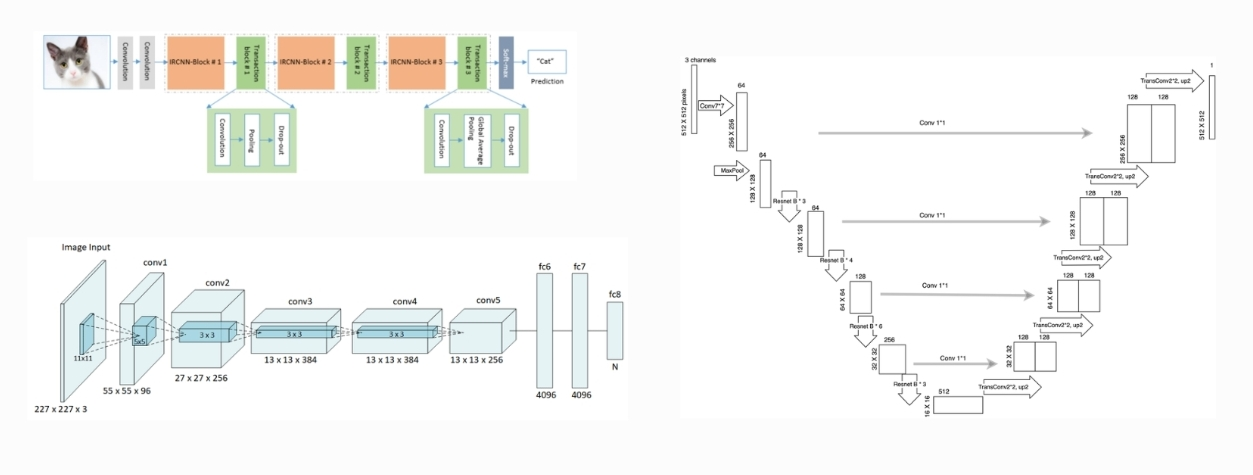
\includegraphics[width=0.8\textwidth]{img/different_types_of_cnn_nets.jpg}
            \caption{Verschiedene Architekturen von Image Networks. Oben links vereinfachtest Alex net, unten links inception net, rechts Abbildung der Res net Architektur.}
            \label{fig:my_label}
        \end{figure}
        
        AlexNet\footfullcite{Aloysius2017} war das erste CNN, das auf einem großen Datensatz erfolgreich angewendet wurde.
        ResNet zeichnet sich durch seine Fähigkeit aus, sehr tiefe Netzwerke zu trainieren, ohne dass das Problem des Verschwindens des Gradienten auftritt\footfullcite{Pengcheng2020}.  
        Inception wiederum ist für seine Fähigkeit bekannt, die Effizienz von CNNs durch die Verwendung von sogenannten Inception-Modulen zu erhöhen\footfullcite{Zahangir2017}.
        %TODO Grafiken für die Netzwerke raussuchen (BV Vorlesung?)

        \begin{figure}[h]
            \centering
            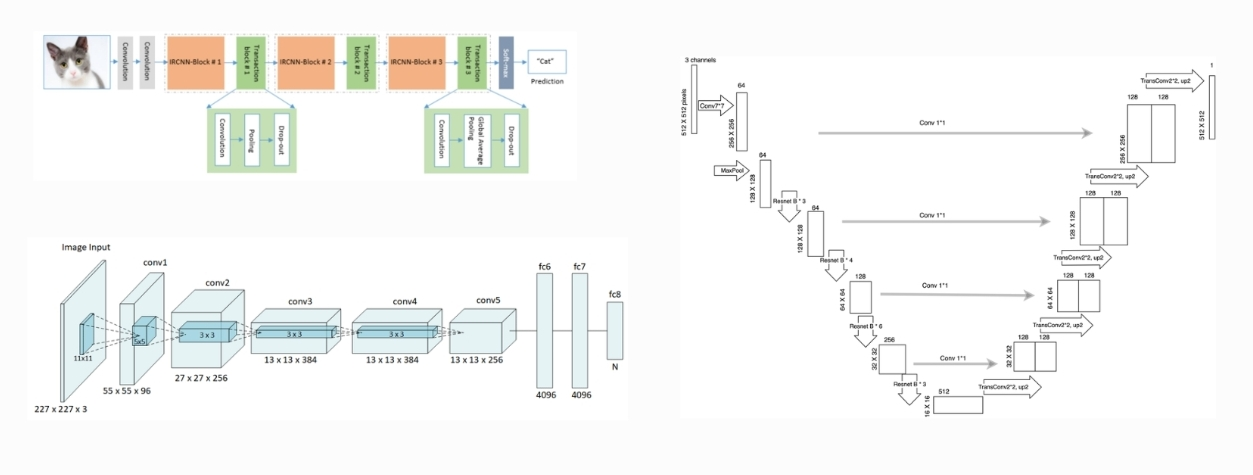
\includegraphics[width=0.8\textwidth]{img/different_types_of_cnn_nets.jpg}
            \caption{Verschiedene Architekturen von Image Networks. Oben links vereinfachtest Alex net, unten links inception net, rechts Abbildung der Res net Architektur.}
            \label{fig:my_label}
        \end{figure}
        
        AlexNet\footfullcite{Aloysius2017} war das erste CNN, das auf einem großen Datensatz erfolgreich angewendet wurde.
        ResNet zeichnet sich durch seine Fähigkeit aus, sehr tiefe Netzwerke zu trainieren, ohne dass das Problem des Verschwindens des Gradienten auftritt\footfullcite{Pengcheng2020}.  
        Inception wiederum ist für seine Fähigkeit bekannt, die Effizienz von CNNs durch die Verwendung von sogenannten Inception-Modulen zu erhöhen\footfullcite{Zahangir2017}.
    
    \subsection{Anwendungen von CNNs}
    
        CNNs haben zahlreiche Anwendungen, darunter Bildklassifizierung, Objekterkennung und Gesichtserkennung.      
        Bei der Bildklassifizierung werden Bilder automatisch in verschiedene Kategorien eingeteilt.      
        Beispielsweise können Bilder in Klassen wie Hunde, Katzen oder Autos eingeteilt werden.  
        Bei der Objekterkennung wird das Modell darauf trainiert, bestimmte Objekte in einem Bild zu erkennen, wie z.B.      Personen oder Straßenschilder.      
        Die Gesichtserkennung wird oft zur Identifikation von Personen in Sicherheitsanwendungen eingesetzt.
        \footfullcite{wu2017squeezedet,liu2015deep,jaderberg2015spatial}\footnote{\url{https://www.researchgate.net/figure/Object-detection-in-a-dense-scene_fig4_329217107}}

        \begin{figure}[h]
            \centering
            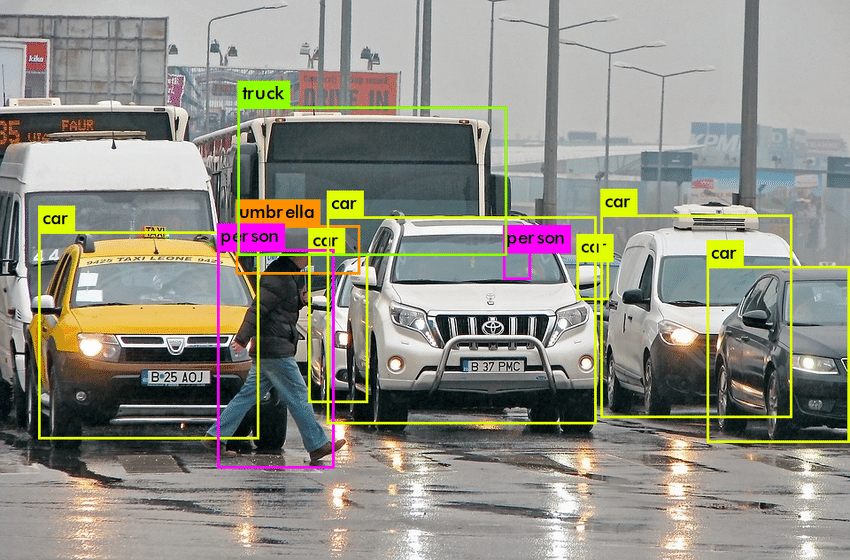
\includegraphics[width=0.6\textwidth]{img/Object-detection-in-a-dense-scene.ppm.png}
            \caption{Beispielbild eines Frames mit Bounding Boxes}
            \label{fig:Beispielbild_eines_Frames_mit_Bounding_Boxes}
        \end{figure}


    \subsection{Transfer Learning mit CNNs}
    
        Transfer Learning ist eine Technik, bei der ein bereits trainiertes CNN auf eine neue Aufgabe angewendet wird, ohne es von Grund auf neu zu trainieren.      
        Dies ist nützlich, wenn man nur über begrenzte Trainingsdaten verfügt oder wenn das Trainieren eines neuen Modells zu viel Zeit oder Ressourcen in Anspruch nimmt.      
        Ein Beispiel hierfür ist Erkennung von Autos, bei denen das Modell auf einem bereits trainierten CNN basieren kann, das auf z\.B\. Yolo v8 trainiert wurde\footfullcite{Nguyen2021}.

        In unserem Projekt haben wir das Modell resnet50 zur Trainingsgrundlage genommen, um unser eigenes Modell zu entwickeln. Wir haben den Code, den wir verwendet haben, um dieses Training durchzuführen, im Folgenden aufgeführt:

        \begin{lstlisting}
Net = torchvision.models.segmentation.deeplabv3_resnet50(pretrained=True)
        \end{lstlisting}

        Dieser Code\footnote{\url{https://github.com/studienarbeit-cnn-dhbwka-2022/Segmentation_cnn/blob/main/cnn.ipynb}} ermöglichte es uns, die Leistungsfähigkeit von resnet50 auszunutzen und es an unsere spezifischen Anforderungen anzupassen. Durch das Training unseres Modells konnten wir die gewünschten Ergebnisse erzielen und wichtige Erkenntnisse gewinnen, ohne ein Model von Grund auf zu trainieren.
        
    \subsection{Limitationen von CNNs und aktuelle Forschungsziele}

        Obwohl CNNs sehr erfolgreich bei der Verarbeitung von Bildern sind, haben sie auch einige Limitationen.      
        Zum Beispiel sind sie nicht gut geeignet, um komplexe Abhängigkeiten zwischen verschiedenen Eingabemerkmalen zu erfassen, wie z.B. das Verhalten von Objekten in einem Video.
        Zudem benötigen CNNs weiterhin viel Rechenleistung und Ressourcen
        \footfullcite{li2018visualizing}

        Facebooks Segment Anything Model (SAM) ist ein neues und Open-Source Modell, das sowohl interaktive als auch automatische Segmentierung durchführen kann.
        Die Benutzeroberfläche des Modells ermöglicht es, es auf flexible Weise zu verwenden, was eine Vielzahl von Segmentierungsaufgaben durch einfache Ingenieursarbeiten möglich macht.
        Das Modell wurde auf einem Datensatz von 11 Millionen Bildern und 1,1 Milliarden Masken trainiert und hat eine starke Null-Schuss-Leistung bei einer Vielzahl von Segmentierungsaufgaben\footnote{\url{https://research.facebook.com/publications/segment-anything/}}.

        \begin{figure}[h]
            \centering
            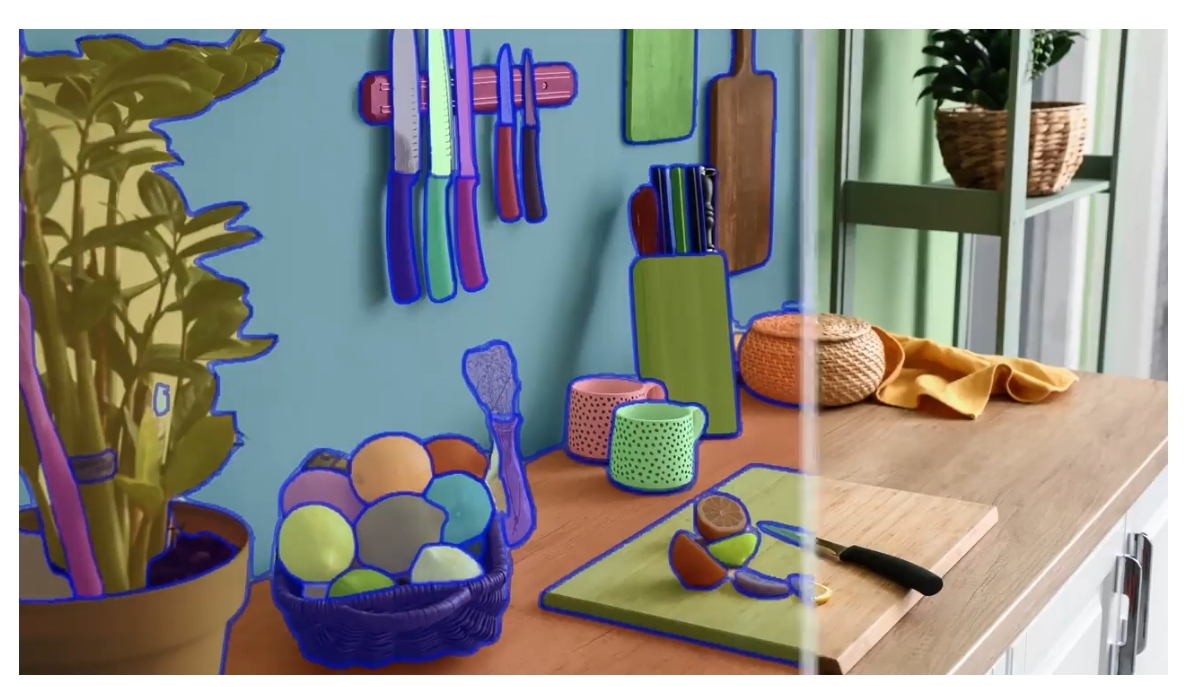
\includegraphics[width=0.6\textwidth]{img/SmartSelect_20230517_135035_Firefox.jpg}
            \caption{SAM: A generalized approach to segmentation}
            \label{fig:facebook_sam}
        \end{figure}

\section{Super Resolution}
    \subsection{Grundlagen von Super Resolution }
    
        Super Resolution \ac{SR} ist eine Technik, um aus einer niedrig aufgelösten Eingabe ein hochauflösendes Bild zu generieren.      
        Dies wird oft als Upscaling bezeichnet und findet in vielen Anwendungen wie der Bildrekonstruktion und Videoanalyse Anwendung.
        Die Grundidee hinter SR ist, dass hochauflösende Informationen in einem niedrig aufgelösten Bild versteckt sein können.      
        Die Herausforderung besteht darin, diese Informationen zu extrahieren und in ein hochauflösendes Bild zu integrieren.      
        SR ist somit ein Problem der inversen Bildgebung, bei dem eine hohe Auflösung aus einer niedrigen Auflösung abgeleitet werden muss.
        \footfullcite{7115171}
        
    \subsection{Super Resolution-Methoden auf Basis von Deep Learning}
    
        Super Resolution-Methoden auf Basis von Deep Learning haben in den letzten Jahren viel Aufmerksamkeit erhalten und sind derzeit der Stand der Technik für SR.      
        Diese Methoden verwenden Convolutional Neural Networks (CNNs) zur Verarbeitung von Bildern und zur Generierung von hochauflösenden Bildern.
        Es gibt verschiedene Arten von SR-Methoden auf Basis von Deep Learning, darunter Single-Image Super Resolution (SISR) und Multi-Image Super Resolution (MISR).      
        SISR-Methoden verwenden nur ein niedrig aufgelöstes Bild als Eingabe, während MISR-Methoden mehrere Bilder verwenden, um ein hochauflösendes Bild zu generieren.

        \begin{figure}[h]
            \centering
            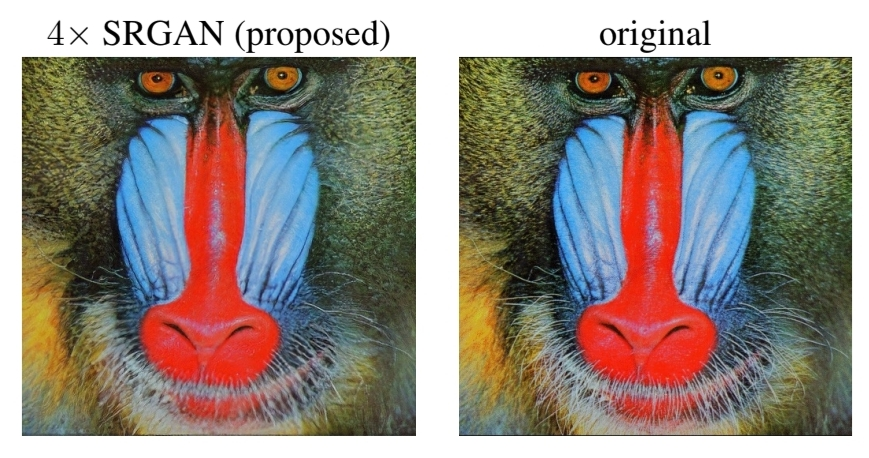
\includegraphics[width=0.7\textwidth]{img/SmartSelect_20230517_140120_Samsung Notes.jpg}
            \caption{Super resolution links, original rechts}
            \label{fig:superresolution}
        \end{figure}
        
        %TODO mehr auf sisr und misr eingehen hab ich aber nur semi verstanden so far 
    
    \subsubsection{Anwendungen von SR}
    
        SR hat viele Anwendungen in der Bild- und Videoanalyse, einschließlich der Rekonstruktion von Bildern aus medizinischen Scans, der Verbesserung von Bildern für die forensische Analyse\footfullcite{10.1007/978-0-387-73742-3_20} und der Verbesserung von Bildern für die Erkennung von Gesichtern und Objekten.
        In der Videoanalyse kann SR verwendet werden, um Videos zu stabilisieren, indem Bewegungsunschärfe reduziert und die Schärfe der Bilder verbessert wird.      
        SR kann auch bei der Entschlüsselung von unscharfen und verschwommenen Bildern in Überwachungsaufnahmen helfen.
    
    \subsubsection{Evaluierung von SR-Methoden}
    
        Die Evaluierung von SR-Methoden ist eine wichtige Aufgabe, um die Qualität und Effektivität der generierten Bilder zu bestimmen.      
        Die gängigen Evaluierungsmethoden umfassen die Verwendung von visuellen Qualitätsmetriken wie Peak Signal-to-Noise Ratio (PSNR) und Structural Similarity Index Measure (SSIM).
        Es gibt auch speziellere Evaluierungsmethoden wie die Verwendung von Perceptual Quality Assessment (PQA)-Maßnahmen, die menschliche Wahrnehmungseigenschaften berücksichtigen, um die Qualität der generierten Bilder zu bestimmen.
    
    \subsubsection{Herausforderungen und zukünftige Forschungsziele von Super Resolution}
    
        Obwohl SR-Methoden auf Basis von Deep Learning vielversprechende Ergebnisse erzielt haben, gibt es immer noch Herausforderungen und zukünftige Forschungsziele, die erforscht werden müssen.
        Eine der Herausforderungen besteht darin, dass SR-Methoden häufig dazu neigen, Artefakte in den generierten Bildern zu erzeugen, insbesondere bei der Verwendung von sehr hohen Upscaling-Faktoren.      %TODO Beispielbild Artefakte erklären
        Dies kann die visuelle Qualität der generierten Bilder beeinträchtigen und die Anwendbarkeit von SR-Methoden in bestimmten Szenarien einschränken.
        
        Eine weitere Herausforderung besteht darin, dass SR-Methoden häufig sehr rechenaufwändig sind, insbesondere wenn sie auf großen Datensätzen oder in Echtzeit angewendet werden müssen.      
        Die benötigten Ressourcen sind teuer.
        Dies kann die praktische Anwendbarkeit von SR-Methoden in einigen Anwendungen einschränken.        
        Zukünftige Forschungsziele könnten sich darauf konzentrieren, diese Herausforderungen zu überwinden, indem sie neue SR-Methoden entwickeln, die sowohl effektiv als auch effgizient sind.      
        Eine mögliche Lösung wäre die Verwendung von Generative Adversarial Networks (GANs) zur Verbesserung der visuellen Qualität der generierten Bilder und zur Reduzierung von Artefakten.      %TODO näher auf GAN eingehen 
        Eine weitere mögliche Lösung wäre die Entwicklung von neuartigen Architekturen von Deep Learning-Netzwerken, die weniger rechenaufwändig sind und schneller ausgeführt werden können\footfullcite{dong2016accelerating}\footfullcite{Park2020}.

        \subsubsection{Deep Learning Super Sampling}

        Eine vielversprechende Lösung zur Beschleunigung von Deep Learning ist Nvidia's DLSS-3 (Deep Learning Super Sampling 3, Stand 2023 Mai 17)\footnote{\url{https://www.nvidia.com/en-us/geforce/news/dlss3-ai-powered-neural-graphics-innovations/}}. 
        DLSS ist eine fortschrittliche Technologie, die von NVIDIA entwickelt wurde und es ermöglicht, hochauflösende Grafiken in Echtzeit zu rendern, indem es auf KI-Methoden basiert und durch Hardware (GPU) beschleunigt wird.
        DLSS bietet nicht nur schnellere Renderzeiten, sondern ermöglicht auch eine verbesserte Leistung auf Grafikkarten, da weniger rechenintensive Berechnungen erforderlich sind.
        Durch extensive Nutzung der CUDA cores, welche immer imposanter in Grafikarten eingebaut werden, ist das berechnen von Hohchauflösenden Bilder schneller mit jeder generation.
            
        % I want a tea party with Y'ha-nthlei

        ~
        
        Insgesamt bleibt SR ein aktives Forschungsfeld mit großem Potenzial für Anwendungen in der Bild- und Videoanalyse.      
        Mit weiteren Fortschritten in der Forschung können SR-Methoden immer leistungsfähiger und praktischer werden, um die Bedürfnisse der Industrie und der Geselllschaft zu erfüllen.

\section{Generative Adversarial Networks (GANs)}

    \subsection{Grundlagen von Generative Adversarial Networks (GANs)}
        
        Generative Adversarial Networks (GANs) sind ein leistungsstarkes Framework für das Training von Deep Learning-Modellen zur Generierung von Daten.      
        GANs bestehen aus zwei miteinander konkurrierenden neuronalen Netzwerken, einem Generator und einem Diskriminator.

        \begin{figure}[h]
            \centering
            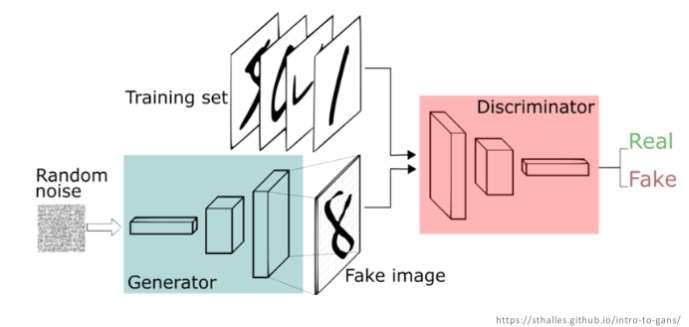
\includegraphics[width=0.7\textwidth]{img/GAN_architecture.jpg}
            \caption{Der Generator erzeugt neue Daten, während der Diskriminator versucht, zwischen den vom Generator erzeugten Daten und den echten Daten zu unterscheiden.}
            \label{fig:GAN_aufbau}
        \end{figure}
        
        Im Laufe des Trainings passt sich der Generator kontinuierlich an und verbessert seine Fähigkeit, realistische Daten zu generieren, während der Diskriminator gleichzeitig verbessert wird, um zwischen den generierten und echten Daten zu unterscheiden.
        %TODO GRAFIK! LUKAS! GRAFIK!
    
    \subsection{Architekturen von GANs}
    
        Es gibt verschiedene Architekturen von GANs, die für verschiedene Arten von Anwendungen geeignet sind.      
        in Beispiel ist das Deep Convolutional GAN (DCGAN), das speziell für die Generierung von Bildern entwickelt wurde.      %TODO Bild? ALso so architekkturbild oder so idk
        DCGAN nutzt Convolutional Neural Networks (CNNs) und Transposed Convolutional Neural Networks, um Bilder zu generieren, die visuell realistisch aussehen und strukturell konsistent sind.
        Ein weiteres Beispiel ist das CycleGAN\footfullcite{CycleGAN2017}, das für die Bildübersetzung zwischen verschiedenen Domänen verwendet werden kann.      
        CycleGAN nutzt einen Generator und einen Diskriminator sowie zusätzliche Cycle-Verlustfunktionen, um die Transformationen zwischen den Bildern in verschiedenen Domänen zu erlernen.%todo quellen vergessen
    
    \subsection{Anwendungen von GANs}
    
        GANs finden Anwendungen in verschiedenen Bereichen wie der Bildgenerierung, Style Transfer, der Verbesserung von Bildern und der Videoanalyse.      
        Zum Beispiel können GANs verwendet werden, um realistisch aussehende Bilder von Gesichtern, Landschaften oder anderen Objekten zu generieren.

        \begin{figure}[h]
            \centering
            
\includegraphics[width=0.4\textwidth]{img/cactus.jpg}
            \caption{Eingabe in das Modell: A small cactus wearing a straw hat and neon sunglasses in the Sahara desert.: \url{https://imagen.research.google/}}
            \label{fig:GAN_example}
        \end{figure}


        Style Transfer ermöglicht die Veränderung des visuellen Erscheinungsbildes von Bildern durch die Übertragung des Stils von einem Bild auf ein anderes.
        Dabei wird ein vortrainiertes neuronales Netzwerk verwendet, um Merkmale des Stils und Inhalts eines Bildes zu erfassen und zu kombinieren.
        Diese Technik hat Anwendungen in der Bildbearbeitung, Kunstgenerierung und visuellen Effekterstellung gefunden.
        
        Durch Style Transfer kann der visuelle Stil eines Bildes auf ein anderes übertragen werden, wobei ein vortrainiertes neuronales Netzwerk die Merkmale des Stils und Inhalts erfasst.
        Dies ermöglicht künstlerische Effekte und Anpassungen in der Bildbearbeitung und eröffnet neue Möglichkeiten für die kreative Gestaltung von visuellen Inhalten.

        Wie im dargestellten Bild zu sehen ist, wird das ursprüngliche Bild mithilfe des Stils des Gemäldes übertragen, wobei die Konturen des Hundes weiterhin erkennbar bleiben.

        \begin{figure}[h]
            \centering
            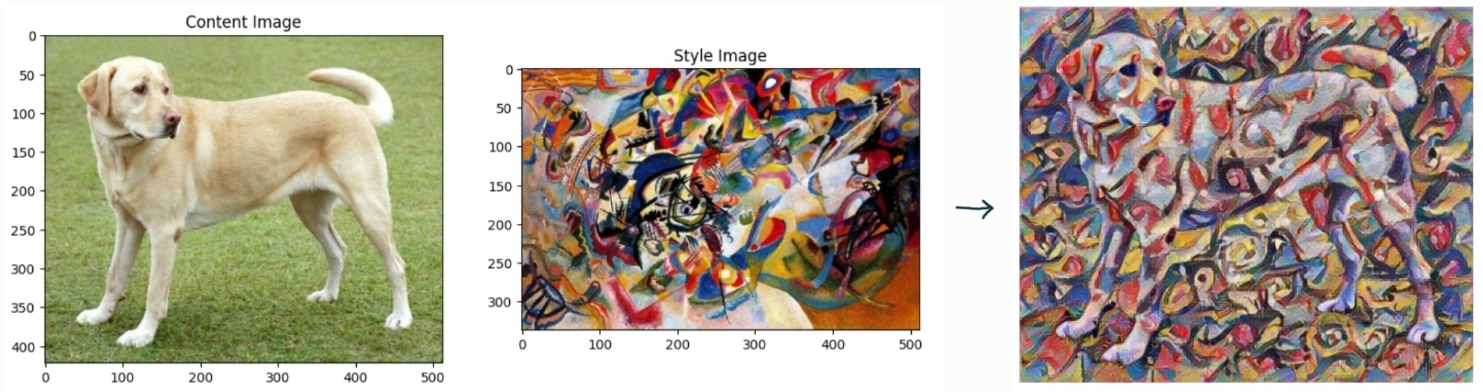
\includegraphics[width=0.9\textwidth]{img/GAN_style_trtansfer.jpg}
            \caption{\url{https://www.tensorflow.org/tutorials/generative/style_transfer}}
            \label{fig:GAN_style_transfer}
        \end{figure}
        
        GANs können auch verwendet werden, um Bilder mit höherer Auflösung oder besserer Qualität zu generieren, indem sie niedrig aufgelöste Bilder als Eingabe verwenden.
        GANs werden immer öfters in Bildverabreitungstools eingesetzt um fehlende Bereiche zu füllen, oder zum erweitern von Bildern (siehe \ref{fig:extend_image_imagen})\footnote{\url{https://imagen.research.google/}}.

        \begin{figure}[!h]
          \centering
          \begin{minipage}[b]{0.6\textwidth}
            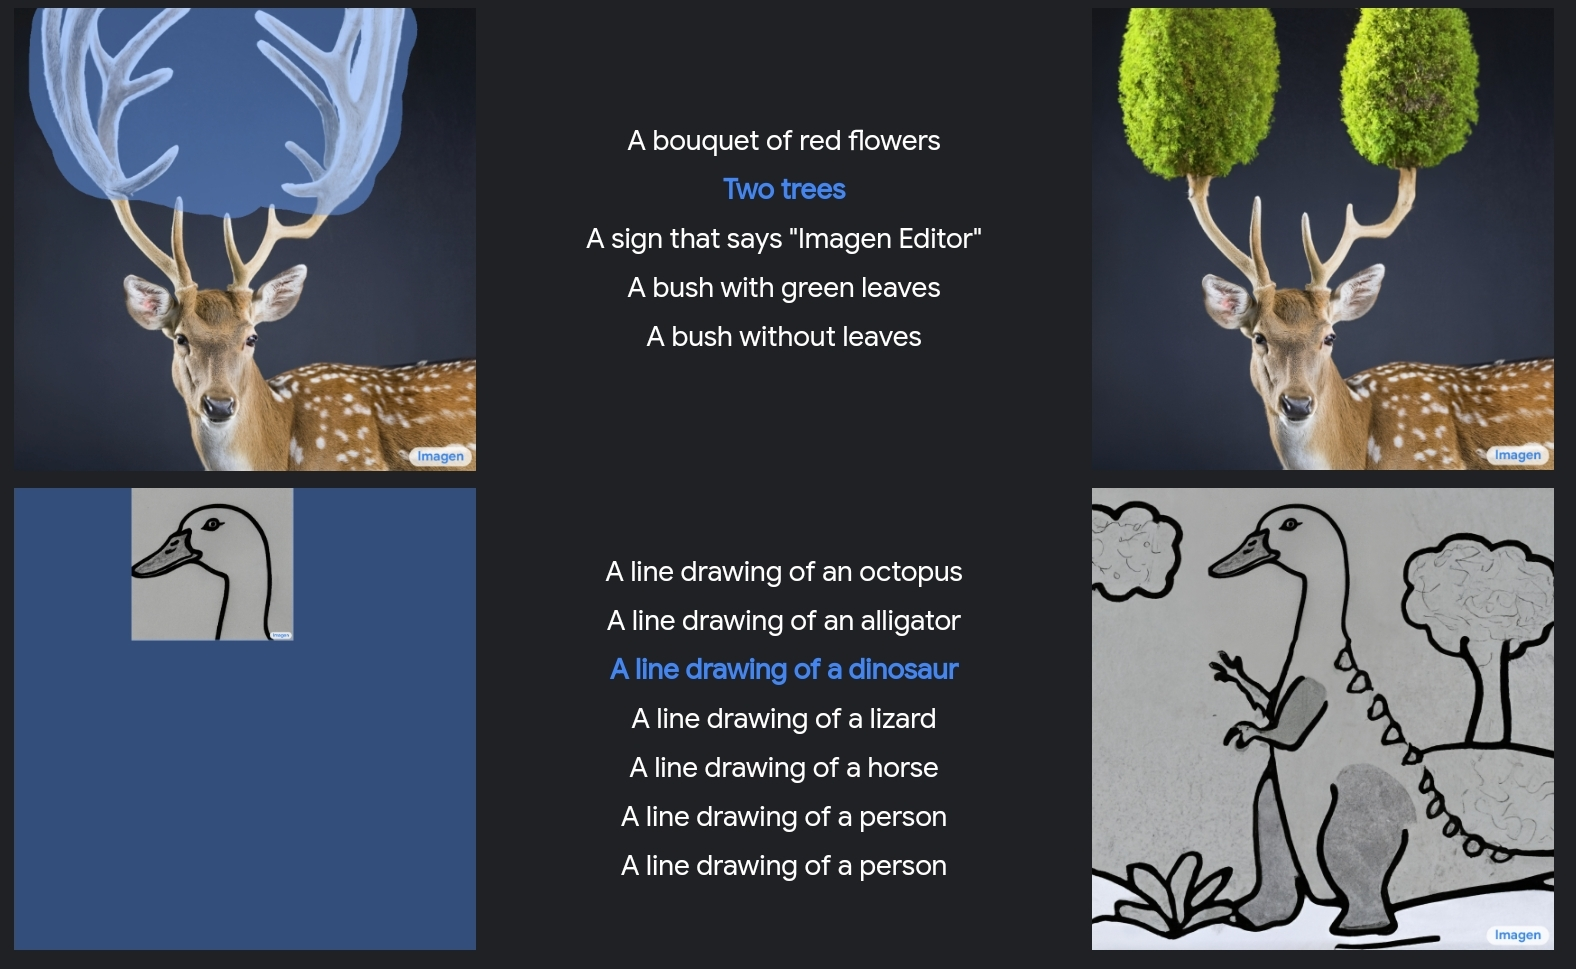
\includegraphics[width=\textwidth]{img/imagen_google_fill_and_extend.jpg}
          \end{minipage}
          \hfill
          \begin{minipage}[b]{0.35\textwidth}
            \caption{Füllen von markierten Bereichen eines Bildes durch verwendung von Imagen und Erweitern von Bildern mithilfe von Imagen, Google.}
          \end{minipage}
          \label{fig:extend_image_imagen}
        \end{figure}

        \newpage 
        % I cant deal with stupid latex anymore. Icant ocant icant

        In der Forschung können GANs verwendet werden, um Videosequenzen zu generieren oder zu verbessern. Ein modernes beispiel wäre Facebooks errungenschaften durch Make-A-Video\footnote{\url{https://ai.facebook.com/blog/generative-ai-text-to-video/}}, siehe \ref{fig:facebook_make_a_video}.

        \begin{figure}[!h]
            \centering
            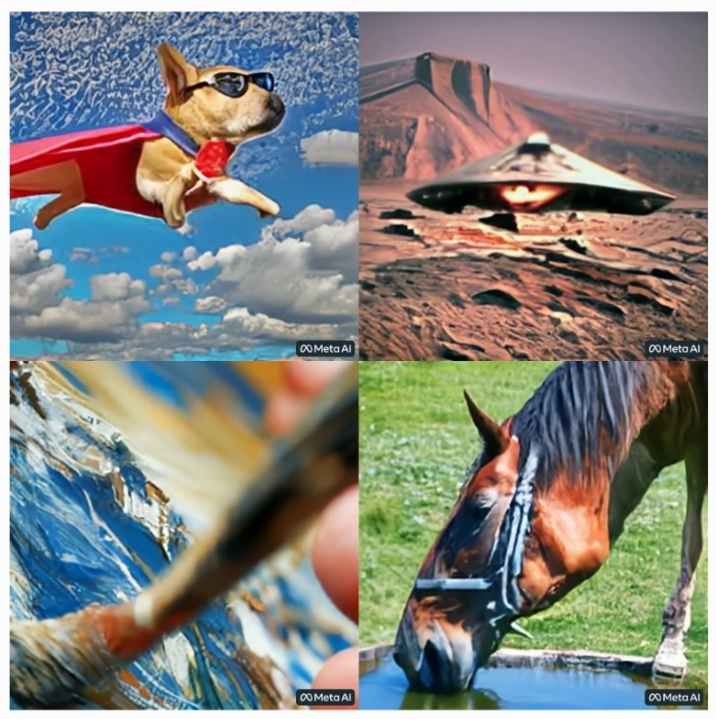
\includegraphics[width=0.6\textwidth]{img/facebook_make_a_video.jpg}
            \caption{Generierung kurzer Videos, anhand von sehr einfachen Beschreibungen.}
            \label{fig:facebook_make_a_video}
        \end{figure}
        
        Da wir leider nicht in Hogwards leben\footnote{Interaktive Zeitung aus Harry Potter: \url{https://youtu.be/xaBEFqFVSE8}}, können Videos \textit{nicht} auf PDFs angezeigt werden, noch weniger auf Papier. Die Eingaben für das Modell sind wie folgt: 
        Oben Links: A dog wearing a superhero cape flying through the sky.
        Oben rechts: A spaceship landing on Mars.
        Unten links: An artist's brush painting on a canvas close up, highly detailed. 
        Unten rechts: A horse drinking water.
        

    \subsection{Training von GANs und Evaluierung von generierten Ergebnissen}

        Das Training von GANs ist eine Herausforderung, da es sich um ein adversariales Lernverfahren handelt.      
        Das bedeutet, dass es zwei Netze gibt, die sich gegenseitig trainieren und verbessern.      %TODO Grafik & Quellen
        % Nö

        ~
        
        Das generative Netzwerk versucht, Bilder zu erzeugen, die von einem diskriminierenden Netzwerk nicht von echten Bildern unterschieden werden können.      
        Das diskriminierende Netzwerk wird trainiert, um echte Bilder von den vom generativen Netzwerk generierten Bildern zu unterscheiden.
        Das Training von GANs erfolgt durch die Minimierung einer Verlustfunktion, die als GAN-Verlust bezeichnet wird.

        ~
        
        Der GAN-Verlust besteht aus zwei Komponenten: dem Verlust des generativen Netzes und dem Verlust des diskriminierenden Netzes.      
        Der Verlust des generativen Netzes wird minimiert, wenn dasd Netzwerk Bilder erzeugt, die vom diskriminierenden Netzwerk nicht als gefälscht erkannt werden.      
        Der Verlust des diskriminierenden Netzes wird minimiert, wenn das Netzwerk in der Lage ist, besonders zuverlässig und schnell zwischen echten und generierten Bildern zu unterscheiden.
        Die Evaluierung von generierten Ergebnissen ist eine wichtige Aufgabe bei der Arbeit mit GANs.

~

        Es gibt verschiedene Methoden zur Bewertung von GANs, wie beispielsweise die visuelle Bewertung, die qualitative Bewertung und die quantitative Bewertung.  
        Die visuelle Bewertung beinhaltet das Betrachten der generierten Bilder, um zu beurteilen, ob sie realistisch aussehen oder nicht.      
        Die qualitative Bewertung beinhaltet die Verwendung von Bewertungsskalen, um die Qualität der generierten Bilder zu bewerten.      
        Die quantitative Bewertung beinhaltet die Verwendung von Metriken wie der Inception Score oder der Frechet Inception Distance, um die Qualität der generierten Bilder zu bewerten.

    \subsection{Ethische und soziale Implikationen von GANs}

    \begin{center}
        \textit{There are several ethical challenges facing text-to-image research broadly. We offer a more detailed exploration of these challenges in our paper and offer a summarized version here. First, downstream applications of text-to-image models are varied and may impact society in complex ways.}

        \url{https://imagen.research.google/}
    \end{center}
    
        Obwohl GANs eine vielversprechende Technologie sind, gibt es auch ethische und soziale Implikationen, die berücksichtigt werden müssen.      
        Ein Problem bei der Verwendung von GANs ist, dass sie zur Erzeugung gefälschter Bilder oder Videos verwendet werden können.      
        Dies kann zu Fälschungen und Manipulationen führen, die negative Auswirkungen auf die Gesellschaft haben können.
        Auch Rufschädigung kann durch GANs errleichtert werden.
        Ein weiteres Problem bei der Verwendung von GANs ist, dass sie möglicherweise nicht fair sind.  

        ~

        GANs können aufgrund ihrer Lernmethode unbewusste Vorurteile aufnehmen und in ihren generierten Ergebnissen widerspiegeln.      
        Dies kann zu diskriminierenden Ergebnissen führen, die unfaire Entscheidungen unterstützen.
        Es ist wichtig, dass bei der Verwendung von GANs Ethik und soziale Verantwortung berücksichtigt werden.      
        Es sollten Maßnahmen ergriffen werden, um sicherzustellen, dass GANs fair und ethisch korrekt arbeiten.      
        Zum Beispiel können spezielle Algorithmen entwickelt werden, um unbewusste Vorurteile zu minimieren.      
        Weiterhin können Regierungsbehörden und andere Organisationen Maßnahmen ergreifen, um den Missbrauch von GANs zu verhindern.   
        Das finden eines Kompromiss aus Forschung und politischer Einschränkung übersteigt jedoch den Rahmen dieser Arbeit.      
    
\section{Multiskalenskalierun}

    In vielen Anwendungen der Bildverarbeitung und Computergrafik ist es notwendig, Objekte oder Strukturen in verschiedenen Größenordnungen zu analysieren oder darzustellen.      
    Multiscale-Skalierung bezeichnet Techniken und Vorgehen, die es ermöglichen, Objekte oder Signale auf verschiedenen Skalen zu untersuchen oder zu manipulieren.      
    Dabei können sowohl lokale als auch globale Eigenschaften eines Objekts berücksichtigt werden.
    Diese Möglichkeiten komplementieren häufig Implementierungen von künstlichen Intelligenzen
    %TODO Zitat richtig einbauen

    \begin{center}
        \textit{Machine learning and multiscale modeling mutually complement one another.}\footfullcite{alber2019integrating}
    \end{center}
    
    \begin{center}
        \textit{Machine learning and multiscale modeling mutually complement one another.}\footfullcite{alber2019integrating}
    \end{center}
    
    \subsection{Grundlagen von Multiskalenskalierung}
    
        Multiscale-Skalierung ist ein Konzept aus der Signal- und Bildverarbeitung, das auf der Idee basiert, dass Signale und Bilder aus verschiedenen Skalen von Strukturen aufgebaut sind.
        In der Praxis bedeutet dies, dass ein Signal oder Bild auf verschiedene Skalen abgetastet oder transformiert wird, um Informationen auf verschiedenen Größenskalen zu erhalten.
        Ein grundlegendes Konzept der Multiscale-Skalierung ist die Skaleninvarianz.      
        Das bedeutet, dass die Informationen in einem Signal oder Bild unabhängig von der Skala erhalten bleiben sollten.      
        Das heißt, dass dieselben Merkmale oder Strukturen auf verschiedenen Skalen erkennbar sein sollten.
        \footfullcite{mallat1989theory,huang2017densely}
    
    \subsection{Methoden zur Multiskalenanalyse}
    
        Es gibt verschiedene Techniken zur Multiskalenanalyse, darunter Wavelet-Transformation und pyramidenartige Strukturen.      
        Wavelet-Transformation ist eine Methode zur Analyse und Synthese von Signalen oder Bildern auf verschiedenen Skalen.      
        Dabei wird das Signal oder Bild auf verschiedene Skalen und Frequenzen zerlegt, um Informationen auf verschiedenen Skalen zu erhalten.
        Pyramidenartige Strukturen sind eine weitere Methode zur Multiskalenanalyse, die in der Bildverarbeitung häufig verwendet wird.      
        Dabei wird das Signal oder Bild auf verschiedenen Skalen durch wiederholte Subsampling- und Filterungsoperationen reduziert.      
        Auf jeder Ebene der Pyramide wird das Signal oder Bild auf eine kleinere Größe reduziert, um Informationen auf verschiedenen Skalen zu erhalten.
        \footfullcite{burt1987laplacian,nah2017deep}
    
    \subsection{Methoden zur Multiskalenanalyse}
        Es gibt verschiedene Methoden zur Multiskalenanalyse, darunter Wavelets und Pyramiden.      
        Wavelets basieren auf der Zerlegung von Signalen in unterschiedliche Frequenzbänder, wodurch eine Multiskalenanalyse ermöglicht wird.      
        Eine Wavelet-Transformation kann auf ein Signal angewendet werden, um es in seine Hoch- und Niederfrequenzkomponenten zu zerlegen.      
        Diese Komponenten können dann unabhängig voneinander verarbeitet werden, um eine Analyse auf verschiedenen Skalen durchzuführen.
        Pyramiden sind eine weitere Methode zur Multiskalenanalyse, die auf der Idee der rekursiven Unterteilung von Signalen in immer feinere Skalen basiert.      Dabei wird ein Signal in eine Pyramide aus verschiedenen Ebenen unterteilt, wobei jede Ebene eine andere Skala darstellt.      
        Die unterste Ebene enthält das Originalsignal, während die oberen Ebenen eine immer gröbere Approximation des Signals enthalten.
        \footfullcite{simoncelli1996noise}
    
    \subsection{Anwendungen von Multiscale-Skalierung}
        Multiscale-Skalierung hat viele Anwendungen in der Bildverarbeitung und Computer Vision.
        Ein Beispiel ist die Texturanalyse, bei der Texturen auf verschiedenen Skalen analysiert werden, um Muster und Strukturen zu identifizieren.      
        Multiscale-Skalierung wird auch in der Bildkompression verwendet, um Bilder auf verschiedene Auflösungen zu skalieren und so Speicherplatz zu sparen.
        In jüngerer Zeit wurde die Multiskalenanalyse auch in Verbindung mit Deep Learning eingesetzt, um Modelle zu entwickeln, die auf verschiedenen Skalen arbeiten können.      
        Ein Beispiel ist das Multiscale Dense Network \ac{MSDN}, das eine skalierbare Architektur für die Bilderkennung bietet, die auf mehreren Skalen arbeiten kann.
    
    \subsection{Limitierungen und zukünftige Forschungsziele von Multiscale-Skalierung}
        Obwohl die Multiskalenanalyse in vielen Bereichen der Bildverarbeitung und Computer Vision erfolgreich eingesetzt wurde, gibt es auch einige Limitationen.  
        Eines der Hauptprobleme ist die Herausforderung, die richtige Skala für eine bestimmte Aufgabe zu wählen.      

        
        In einigen Fällen kann dies schwierig sein, da verschiedene Skalen unterschiedliche Informationen enthalten.
        Eine weitere Herausforderung besteht darin, die Multiskalenanalyse mit Deep Learning-Methoden zu integrieren.      
        Während einige Fortschritte in diesem Bereich gemacht wurden, gibt es immer noch Raum für Verbesserungen, um die Multiskalenanalyse nahtlos in Deep Learning-Architekturen zu integrieren\footfullcite{he2016deep}.
        
        Zukünftige Forschungsrichtungen könnten sich auf die Entwicklung von verbesserten Methoden zur Skalierung und Multiskalenanalyse konzentrieren, die eine höhere Genauigkeit und Effizienz ermöglichen.      
        Darüber hinaus könnten Forscher daran arbeiten, die Integration der Multiskalenanalyse in Deep Learning-Architekturen weiter zu verbessern, um noch bessere Ergebnisse zu erzielen.

\section{Vor- und Nachteile der fortgeschrittenen Methoden}

    Im Hinblick auf die Bildqualität sind Deep-Learning-basierte Methoden wie Super Resolution und GANs den traditionellen Methoden wie der Bilinear-Interpolation überlegen.      
    Diese Methoden können hochwertige Bilder mit hoher Auflösung und Details erzeugen, die den Originalbildern nahe kommen.      
    Insbesondere die GANs erlauben die Erzeugung von realistisch aussehenden Bildern, die schwer von echten Bildern zu unterscheiden sind.
    Ein weiterer Vorteil der fortgeschrittenen Methoden ist ihre Fähigkeit zur Generierung von neuen Inhalten.   
    So können GANs und Style Transfer genutzt werden, um neue Bilder zu erzeugen, die auf den Stil und Inhalt anderer Bilder basieren.      
    Dies bietet neue kreative Möglichkeiten in der Kunst und Design.

    Jedoch stellen diese fortgeschrittene Methoden auch Herausforderungen bei der Anwendung dar.      
    Beispielsweise benötigen Deep-Learning-Methoden große Datensätze und Rechenleistung, um optimal zu funktionieren\footfullcite{li2021beginner}.      
    Ein weiteres Problem ist die Interpretierbarkeit\footfullcite{he2023segmentation} der Ergebnisse, da es schwierig sein kann, zu verstehen, wie ein Modell zu seinen Ergebnissen gekommen ist.
    Die Anwendung von fortgeschrittenen Skalierungsmethoden hat auch Auswirkungen auf die Leistung und Effizienz von Systemen\footfullcite{Wang2018}.      
    So können Deep-Learning-basierte Methoden in Echtzeit-Anwendungen, wie beispielsweise autonomen Fahrzeugen, zu Verzögerungen führen.      
    Es ist daher wichtig, dass die Anforderungen an Leistung und Effizienz bei der Auswahl der Skalierungsmethode berücksichtigt werden.
    
    Es gibt moderne Architekturen und Techniken für höchst effiziente und leistungsstarke Ergebnisse.
    Zukunftsaussichten für fortgeschrittene Skalierungsmethoden liegen in der Kombination verschiedener Methoden. 
    So können beispielsweise GANs und Super Resolution zusammen genutzt werden, um qualitativ hochwertige und realistisch aussehende Bilder zu erzeugen.      
    Ein weiteres Forschungsgebiet ist die Verbesserung der Interpretierbarkeit und Erklärbarkeit von Deep-Learning-Modellen.      
    
    Insgesamt bieten fortgeschrittene Skalierungsmethoden in der Bildverarbeitung und Computergrafik viele Vorteile, jedoch müssen auch die Herausforderungen bei der Anwendung und die Auswirkungen auf die Leistung und Effizienz von Systemen berücksichtigt werden\footfullcite{Klver2022}.      
    Zukünftige Forschung sollte darauf abzielen, die verschiedenen Methoden zu kombinieren und die Interpretierbarkeit von Deep-Learning-Modellen zu verbessern.

\newpage


\chapter{Evaluation von Skalierungsmethoden}

\section{Qualitätsmetriken von Skalierungsmethoden}

    Die Evaluation von Skalierungsmethoden in der Bildverarbeitung bedarf einer facettenreichen Palette an Qualitätsmetriken, welche eine präzise Analyse und Vergleichbarkeit unterschiedlicher Methoden ermöglichen. 
    Im Rahmen dieser Arbeit werden ausgewählte sowie zentrale Qualitätsmetriken für die Bewertung von Skalierungsmethoden erörtert und diskutiert.

    \subsection{\ac{PSNR}}
        Das Peak Signal-to-Noise Ratio \ac{PSNR} ist eine der am häufigsten verwendeten Metriken zur Bewertung der Qualität von Bildern.
        Es misst die Qualität einer Bildrekonstruktion, indem es den Unterschied zwischen einem Originalbild und einem rekonstruierten Bild berechnet und diesen Unterschied durch das maximale Signal (Peak) und das Rauschen (Noise) im Originalbild teilt. 
        Je höher der PSNR-Wert, desto geringer ist der Unterschied zwischen Original- und Rekonstruktionsbildern und desto besser ist die Qualität der Rekonstruktion.
        \footfullcite{wang2004image}
        
        \subsubsection{Definition und Berechnung von \ac{PSNR}}
            Die Definition von PSNR lautet wie folgt:
            \begin{equation}
            PSNR = 20 \log_{10} \left( \frac{MAX_I}{\sqrt{MSE}} \right)
            %TODO prüf mal ob die Formel stimmt. Bin verzweifelt und hab die irwo aus stackoverflow geholt
            \end{equation}

            Dabei ist $MAX_I$ der maximal mögliche Pixelwert des Bildes.
            Bei der Darstellung von Pixeln mit 8 Bits pro Abtastwert ist dieser Wert 255.
            Allgemeiner ausgedrückt: Wenn die Samples mit linearer PCM mit B Bits pro Sample dargestellt werden, ist MAXI $2^B - 1$\footfullcite{wiki:Peak_signal-to-noise_ratio}.

            % wobei Peak der höchste mögliche Wert des Signals ist, der meist auf 255 bei 8-Bit-Graustufenbildern oder 65535 bei 16-Bit-Graustufenbildern gesetzt wird. %nur so semi verstanden aber die Quellen haben da ünbereingestimmt (stackoverflow help me)

            \begin{equation}
                MSE = \frac{1}{n*m} \sum_{i=0}^{n-1} \sum_{i=0}^{m-1} (I(i,j) - K(i,j))^2
            \end{equation}

            Der Mean Squared Error \ac{MSE} ist definiert als der Durchschnitt der quadrierten Unterschiede zwischen jedem Pixel des Originalbildes und dem rekonstruierten Bild.
            Je höher der PSNR-Wert, desto geringer ist der \ac{MSE} und desto besser ist die Qualität der Rekonstruktion.

        %TODO Quelle für Formel (wWill kein Stackoverflow link angeben) 
        \subsubsection{Anwendung von \ac{PSNR} bei der Bewertung von Bildqualität}
            Obwohl \ac{PSNR} eine weit verbreitete Methode zur Bewertung der Qualität von Bildern ist, hat sie auch ihre Limitationen\footfullcite{sheikh2006image}.
            Zum einen berücksichtigt sie nur die Fehler zwischen Original- und Rekonstruktionsbildern und vernachlässigt andere Faktoren wie Bildverzerrungen, die durch Komprimierung oder Filterung entstehen können.
            Zum andern ist der \ac{PSNR}-Wert nicht sensitiv für menschlich wahrgenommene Verzerrungen\footfullcite{mittal2012no}, wie z.B. Farbverschiebungen oder Artefakte.
            Trotz dieser Limitationen bleibt \ac{PSNR} eine wichtige Metrik in der Bildverarbeitung und wird oft in der Praxis verwendet, um die Qualität von Bildrekonstruktionen zu bewerten und zu vergleichen.
            \footfullcite{korhonen2012peak}
    \subsection{Structural Similarity Index Measure (SSIM)}

        Der Structural Similarity Index \ac{SSIM} ist eine Metrik zur Bewertung der strukturellen Ähnlichkeit zwischen einem Originalbild und einem rekonstruierten Bild.
        Im Gegensatz zum PSNR berücksichtigt der \ac{SSIM} nicht nur die Pixelwerte, sondern auch die Struktur und Textur des Bildes.
        Der \ac{SSIM} berechnet die Ähnlichkeit zwischen den beiden Bildern anhand von drei Faktoren: Helligkeit, Kontrast und Struktur. Die Formel zur Berechnung von \ac{SSIM} ist wie folgt:

        \begin{equation}
            \text{SSIM}(x, y) = \frac{{(2\mu_x\mu_y + c_1)(2\sigma_{xy} + c_2)}}{{(\mu_x^2 + \mu_y^2 + c_1)(\sigma_x^2 + \sigma_y^2 + c_2)}}
        \end{equation}

        In dieser Formel repräsentieren \(x\) und \(y\) zwei verglichene Bilder.
        Die \ac{SSIM} misst die strukturelle Ähnlichkeit zwischen diesen Bildern.
        \(\mu_x\) und \(\mu_y\) sind die Mittelwerte von \(x\) und \(y\), während \(\sigma_x^2\) und \(\sigma_y^2\) die Varianzen von \(x\) und \(y\) darstellen.
        \(\sigma_{xy}\) repräsentiert die Kovarianz zwischen \(x\) und \(y\).
        Die Konstanten \(c_1\) und \(c_2\) sind kleine Werte, die zur Stabilisierung der Division hinzugefügt werden
        \footfullcite{chen2011fast}\footfullcite{wiki:Structural_similarity}.


        \subsubsection{Anwendung von SSIM bei der Bewertung von Bildqualität}
        
            \ac{SSIM} wird häufig verwendet, um die Qualität von Bildrekonstruktionen zu bewerten. Es hat sich gezeigt, dass \ac{SSIM} besser als PSNR die wahrgenommene Bildqualität wiederspiegelt.
            Dies liegt daran, dass \ac{SSIM} die strukturelle Ähnlichkeit zwischen den beiden Bildern berücksichtigt, während \ac{PSNR} nur die Differenz der Pixelweite betrachtet.

        \subsubsection{Vorteile von SSIM im Vergleich zu PSNR}
        
            Im Vergleich zum \ac{PSNR} hat \ac{SSIM} mehrere Vorteile. Zum einen berücksichtigt es die strukturelle Ähnlichkeit zwischen den beiden Bildern, was zu einer besseren Bewertung der wahrgenommenen Bildqualität führt.
            Zum anderen ist \ac{SSIM} in der Lage, Verzerrungen zu erkennen, die durch Kompression oder andere Arten von Bildverarbeitung verursacht werden, während \ac{PSNR} dies nicht tut.
        \footfullcite{5596999}
        
        \subsubsection{Limitationen von SSIM}
        
            Obwohl \ac{SSIM} eine bessere Metrik zur Bewertung der Bildqualität als \ac{PSNR} darstellt, hat es auch seine Limitationen.
            \ac{SSIM} ist anfällig für Helligkeits- und Kontrastunterschiede zwischen den beiden Bildern und kann bei der Bewertung von stark komprimierten Bildern ungenau sein.
            Auch bei der Anwendung auf Bilder mit unterschiedlichen Strukturen kann die \ac{SSIM} eine ungenaue Bewertung liefern.
        \footfullcite{1284395}
    \subsection{Mean Opinion Score (MOS)}
        Der Mean Opinion Score \ac{MOS} ist eine subjektive Metrik, die die wahrgenommene Qualität einer Bildrekonstruktion misst.
        MOS basiert auf der Bewertung durch menschliche Beobachter, die gebeten werden, die Qualität von Original- und Rekonstruktionsbildern auf einer Skala von 1 bis 5 oder 1 bis 10 zu bewerten.
        MOS ist eine wichtige Metrik, da sie die subjektive Wahrnehmung der Qualität eines Bildes durch den Betrachter berücksichtigt.
        \footfullcite{sheikh2006image}
        
    \subsection{Peak Signal-to-Noise Ratio der Y-Komponente (PSNR-Y)}
        Die Y-Komponente im YCbCr-Farbraum enthält die Helligkeitsinformationen des Bildes. 
        Das Peak Signal-to-Noise Ratio der Y-Komponente \ac{PSNR-Y} ist eine spezielle Version des \ac{PSNR}, die nur die Helligkeitsinformationen des Originalbildes und des rekonstruierten Bildes berücksichtigt.
        \ac{PSNR}-Y ist eine wichtige Metrik zur Bewertung der Qualität von Skalierungsmethoden für Graustufen- oder Schwarz-Weiß-Bilder.
        Diese Qualitätsmetriken sind wichtigeWerkzeuge für diew Bewertung und den Vergleich von Skalierungsmelthoden in der Bildverarbeitung.
        Es ist jedoch wichtig zu beachten, dass keine einzelne Metrik alle Aspekte der Bildqualität abdeckt. Eine umfassende Bewertung sollte mehrere Metriken kombinieren und auch die subjektive Wahrnehmung 
        \footfullcite{huang2010new}
        
    \subsection{Computational Speed}
    
        Die Wahl einer Skalierungsmethode hängt nicht nur von der Bildqualität, sondern auch von der benötigten Rechenleistung ab. 
        Die Computational Speed ist daher ein wichtiger Faktor bei der Auswahl einer Skalierungsmethode.
        Es gibt verschiedene Methoden zur Messung von Computational Speed, wie z.B. die Messung der benötigten Zeit, um ein Bild zu skalieren oder die Berechnung von \ac{FLOPS}. 
        Eine genauere Messung kann durch die Verwendung von Benchmarks erreicht werden, die es ermöglichen, verschiedene Skalierungsmethoden auf derselben Hardware zu vergleichen.
        Jedoch muss bei der Messung der Computational Speed berücksichtigt werden, dass die Leistung des verwendeten Computers die Ergebnisse beeinflussen kann. 
        Ein schnellerer Computer kann eine Methode schneller ausführen als ein langsamerer Computer. 
        Daher ist es wichtig, die Messungen auf einem vergleichbaren Computer durchzuführen und die Ergebnisse zu normalisieren.
        Ein wichtiger Trade-off besteht zwischen der Bildqualität und der Computational Speed. 
        Eine Methode, die eine höhere Bildqualität liefert, benötigt in der Regel mehr Rechenleistung und ist daher langsamer als eine Methode mit niedrigerer Bildqualität. 
        Es ist daher wichtig, die gewünschte Bildqualität und die verfügbare Rechenleistung abzuwägen und eine Methode zu wählen, die den Anforderungen am besten entspricht. 
        Es können auch Techniken wie progressiver Skalierung verwendet werden, um eine gute Bildqualität mit einer angemessenen Geschwindigkeit zu erreichen.
        \footfullcite{xu2017efficient,choi2019lightweight}
        
    \subsection{Root-Mean-Square Error (RMSE)}
    
        Der Root-Mean-Square Error \ac{RMSE} ist eine Metrik zur Bewertung der Qualität von Bildrekonstruktionen. 
        Ein Nachteil von RMSE ist, dass er nur den Fehler zwischen Pixelwerten betrachtet und keine Berücksichtigung von strukturellen Unterschieden im Bild nimmt. 
        Daher wird RMSE oft in Kombination mit anderen Metriken wie \ac{PSNR} und \ac{SSIM} verwendet, um ein umfassenderes Bild der Bildqualität zu erhalten.
        Abschließend ist zu sagen, dass beider Bewertung von Bildqualität die Wahl der Metrik von der spezifischen Anwendung abhängt. 
        Während \ac{PSNR} und \ac{SSIM} für die Bewertung von Bildern in vielen Anwendungen ausreichend sein können, kann in anderen Fällen die subjektive Wahrnehmung des menschlichen Betrachters durch MOS eine bessere Metrik sein.
        Darüber hinaus ist bei der Wahl einer Skalierungsmethode auch die Messung von Computational Speed und das Abwägen von Trade-offs zwischen Bildqualität und Geschwindigkeit von entscheidender Bedeutung.
        \footfullcite{morad1996role}
        
\section{Kriterien zur Auswahl der Skalierungsmethode} %TODO Hier können wir viele Bilder einbauen um die Vergleichsgrafiken besser zu erklären (@MARC)

    \subsection{Bildvergleich und visuelle Bewertung}
        
        Die Evaluation von Skalierungsmethoden in der Bildverarbeitung erfordert eine umfassende und präzise Analyse verschiedener Kriterien, um die optimale Methode auszuwählen. 
        Ein wesentlicher Aspekt bei dieser Bewertung ist der Bildvergleich und die visuelle Bewertung, die auf der subjektiven Wahrnehmung von menschlichen Beobachtern beruhen.
        Die visuelle Bewertung von Bildern durch menschliche Beobachter ermöglicht eine direkte und subjektive Beurteilung der Bildqualität basierend auf wahrgenommenen visuellen Eigenschaften. 
        Verschiedene Methoden des Bildvergleichs werden eingesetzt, wie beispielsweise der Side-by-Side-Vergleich, bei dem zwei Bilder direkt miteinander verglichen werden, oder der Triple-Stimulus-Test, bei dem ein Originalbild mit zwei rekonstruierten Bildern verglichen wird.
        Diese Methoden des Bildvergleichs und der visuellen Bewertung werden auch bei der Evaluierung von Skalierungsmethoden angewendet. 
        Durch den Vergleich der rekonstruierten Bilder mit dem Originalbild können verschiedene Skalierungsmethoden anhand ihrer visuellen Qualität beurteilt und verglichen werden. 
        dies ermöglicht eine umfangreiche Analyse und eine direkte Gegenüberstellung der unterschiedlichen Methoden.
        Es ist jedoch von entscheidender Bedeutung, die Limitationen und Vorbehalte im Zusammenhang mit der visuellen Bewertung von Bildern zu berücksichtigen. 
        Die subjektive Wahrnehmung kann von Person zu Person variieren und wird auch von anderen Faktoren wie Beleuchtung, Betrachtungsabstand und individuellen Präferenzen beeinflusst. 
        Darüber hinaus können komplexe visuelle Verzerrungen nicht immer präzise durch die visuelle Bewertung erfasst werden. 
        Daher sollten bei der Bewertung von Skalierungsmethoden auch objektive Metriken und weitere Evaluierungskriterien einbezogen werden.
        Insgesamt spielt der Bildvergleich und die visuelle Bewertung eine bedeutende Rolle bei der Evaluierung von Skalierungsmethoden in der Bildverarbeitung.
        Durch die Kombination der subjektiven visuellen Bewertung mit objektiven Metriken können fundierte Entscheidungen getroffen werden, um die optimale Methode gemäß den spezifischen Anforderungen der Anwendung auszuwählen. 
        Die sorgfältige Berücksichtigung der genannten Limitationen trägt dazu bei, zuverlässige und aussagekräftige Ergebnisse zu erzielen und die Qualität von Bildrekonstruktionen bestmöglich zu bewerten.
        \footfullcite{ye2012no,wang2004image,eckert1998perceptual}
    
    \subsection{Effektivität und Effizienz}

        Die Bewertung von Skalierungsmethoden in der Bildverarbeitung erfordert eine umfassende Betrachtung sowohl der Effektivität, also der Bildqualität, als auch der Effizienz, insbesondere der Computational Speed. 
        Es besteht ein inhärenter Trade-off zwischen der erzielten Bildqualität und der benötigten Rechenleistung, der bei der Auswahl der optimalen Skalierungsmethode berücksichtigt werden muss.
        Die Effektivität einer Skalierungsmethode bezieht sich auf die erzielte Bildqualität der rekonstruierten Bilder. 
        Eine Methode, die eine höhere Bildqualität liefert, wird in der Regel auch mehr Rechenleistung benötigen und somit langsamer sein als eine Methode mit geringerer Bildqualität. 
        Daher ist es von großer Bedeutung, die gewünschte Bildqualität und die verfügbare Rechenleistung sorgfältig abzuwägen, um die beste Skalierungsmethode zu wählen.


        \begin{table}[!h]
        \centering
        \begin{tabular}{ccccccc}
            \textbf{Model} & \textbf{PLCC} & \textbf{MAE} & \textbf{RMS} & \textbf{SRCC} & \textbf{KRCC} & \textbf{Computation time} \\ \hline
            PSNR           & 0.9062        & 7.4351       & 9.8191       & 0.8804        & 0.6886        & 1                                     \\
            SSIM           & 0.9253        & 6.9203       & 8.8069       & 0.9014        & 0.7246        & 22.65                                 \\
            MS-SSIM        & 0.8945        & 8.1969       & 10.384       & 0.8619        & 0.6605        & 48.49                                 \\
            SSIMplus       & 0.9732        & 4.3192       & 5.3451       & 0.9349        & 0.7888        & 7.83
        \end{tabular}
        \caption{Leistungsvergleich zwischen PSNR, SSIM, MS-SSIM, VQM, PQR-Tek, DMOS-Tek, JND-VC,
DMOS-VC und SSIMplus einschließlich aller Geräte\footfullcite{Rehman_Zeng_Wang_2015}.}
        \label{tab:Leistungsvergleich}
        \end{table}



        Die Evaluierung der Trade-offs zwischen Effektivität und Effizienz erfordert eine gründliche Analyse der Leistungsmerkmale verschiedener Skalierungsmethoden.
        Hierbei können Kosten-Nutzen-Analysen hilfreich sein, um die Auswirkungen der gewählten Methode auf die Bildqualität und die erforderliche Rechenleistung abzuschätzen. 
        Indem die Kosten in Bezug auf die erzielte Bildqualität bewertet werden, kann die optimale Methode entsprechend den spezifischen Anforderungen des Anwendungsbereichs ausgewählt werden.
        Die Relevanz von Effektivität und Effizienz variiert je nach Anwendungsbereich der Bildverarbeitung. 
        In einigen Fällen, wie beispielsweise medizinischen Bildgebungsverfahren oder hochauflösenden Videoanwendungen, ist eine hohe Bildqualität von größter Bedeutung, selbst wenn dies mit einem höheren Rechenaufwand einhergeht. 
        In anderen Szenarien, wie in Echtzeit-Anwendungen oder mobilen Geräten, kann die Effizienz und die schnelle Verarbeitung der Bilder priorisiert werden, auch wenn dies zu einer gewissen Einbuße der Bildqualität führt.
        Insgesamt ist es von entscheidender Bedeutung, sowohl die Effektivität als auch die Effizienz bei der Wahl der besten Skalierungsmethode zu berücksichtigen. 
        Die richtige Balance zwischen Bildqualität und erforderlicher Rechenleistung zu finden, ermöglicht die optimale Nutzung von Ressourcen und die Erfüllung der spezifischen Anforderungen des jeweiligen Anwendungsbereichs der Bildverarbeitung.
        \footfullcite{zhang2019efficiency}\footfullcite{gu2019comprehensive}\footfullcite{hu2020efficient}

    \subsection{Zukunftsaussichten und Herausforderungen}
    
        Die kontinuierliche Entwicklung von Technologien stellt neue Herausforderungen bei der Evaluierung von Skalierungsmethoden in der Bildverarbeitung dar.
        Fortschritte in der Hardware, wie leistungsstärkere Prozessoren und spezialisierte Beschleuniger, können die Rechenleistung erhöhen und somit neue Möglichkeiten für komplexe Skalierungsalgorithmen eröffnen. Gleichzeitig führen neue Technologien wie Virtual Reality, Augmented Reality und 8K-Bildschirme zu höheren Anforderungen an die Bildqualität und erfordern präzisere Bewertungsmethoden.
        Spezifische Anwendungsbereiche, wie die medizinische Bildgebung oder die Videokompression, stellen weitere Herausforderungen bei der Evaluierung von Skalierungsmethoden dar. 
        In der medizinischen Bildgebung ist die genaue Beurteilung der Bildqualität von entscheidender Bedeutung für die richtige Diagnosestellung und Behandlungsplanung. 
        Hier müssen spezielle Metriken und Evaluierungsverfahren entwickelt werden, um den Anforderungen dieses Bereichs gerecht zu werden. 
        Ebenso erfordert die Videokompression eine sorgfältige Evaluierung der Skalierungsmethoden, um eine ausreichende Qualität der komprimierten Videos zu gewährleisten und gleichzeitig die Effizienz der Kompression zu maximieren.
        Ein vielversprechendes Potenzial für die zukünftige Evaluierung von Skalierungsmethoden liegt in der Anwendung von KI-basierten Evaluierungsmethoden. 
        Durch den Einsatz von maschinellem Lernen und neuronalen Netzwerken können automatisierte Bewertungsalgorithmen entwickelt werden, die die menschliche Wahrnehmung von Bildqualität besser simulieren. 
        Diese KI-basierten Ansätze können eine schnellere und objektivere Evaluierung ermöglichen und den Entwicklungsprozess von Skalierungsmethoden beschleunigen.
        Bei der Bewertung von Skalierungsmethoden sollten jedoch auch ethische und soziale Implikationen berücksichtigt werden. 
        Die Entwicklung von immer leistungsfähigeren Skalierungsmethoden kann auch potenzielle Risiken mit sich bringen, wie zum Beispiel die Manipulation von Bildern oder die Schaffung von gefälschten Inhalten. 
        Es ist daher wichtig, entsprechende Schutzmechanismen zu entwickeln, um den Missbrauch solcher Technologien zu verhindern und die Privatsphäre und Integrität von Personen zu wahren.
        Zusammenfassend lassen sich die Zukunftsaussichten für die Evaluierung von Skalierungsmethoden als vielversprechend betrachten. 
        Durch die Berücksichtigung technologischer Entwicklungen, die Bewältigung spezifischer Herausforderungen in verschiedenen Anwendungsbereichen, die Nutzung von KI-basierten Evaluierungsmethoden und die Beachtung ethischer und sozialer Implikationen können wir die Qualität und Effizienz von Skalierungsmethoden weiter verbessern und gleichzeitig sicherstellen, dass sie verantwortungsvoll und zum Wohl der Gesellschaft eingesetzt werden.
        \footfullcite{zhang2015learning}\footfullcite{blau2018perception}\footfullcite{liu2016ssd,zhang2018split}
\newpage



\clearpage
%%%%%%%%%%%%%%%%%%%%%%%%%%%%%%%%%%%%%%%%%%%%%%%%%%%%%%%%%%%%%%%%%%%%%%%%%%%%%%
%% Descr:       Vorlage für Berichte der DHBW-Karlsruhe, Datei mit Abkürzungen
%% Author:      Prof. Dr. Jürgen Vollmer, vollmer@dhbw-karlsruhe.de
%% $Id: abk.tex,v 1.4 2017/10/06 14:02:03 vollmer Exp $
%% -*- coding: utf-8 -*-
%%%%%%%%%%%%%%%%%%%%%%%%%%%%%%%%%%%%%%%%%%%%%%%%%%%%%%%%%%%%%%%%%%%%%%%%%%%%%%%

\chapter*{Abkürzungsverzeichnis}                   % chapter*{..} -->   keine Nummer, kein "Kapitel"
						         % Nicht ins Inhaltsverzeichnis
% \addcontentsline{toc}{chapter}{Akürzungsverzeichnis}   % Damit das doch ins Inhaltsverzeichnis kommt

% Hier werden die Abkürzungen definiert
\begin{acronym}[DHBW]
  % \acro{Name}{Darstellung der Abkürzung}{Langform der Abkürzung}
 \acro{Abk}[Abk.]{Abkürzung}

 % Folgendes benutzen, wenn der Plural einer Abk. benöigt wird
 % \newacroplural{Name}{Darstellung der Abkürzung}{Langform der Abkürzung}
 \newacroplural{Abk}[Abk-en]{Abkürzungen}

 \acro{H2O}[\ensuremath{H_2O}]{Di-Hydrogen-Monoxid}

 % Wenn neicht benutzt, erscheint diese Abk. nicht in der Liste
 \acro{NUA}{Not Used Acronym}
\end{acronym}
              % Abkürzungsverzeichnis
\listoffigures             % Liste der Abbildungen
\listoftables              % Liste der Tabellen
\lstlistoflistings         % Liste der Listings
\listofequations           % Liste der Formeln

% Ab hier beginnt der Anhang
\appendix
\addcontentsline{toc}{chapter}{Anhang}

\addcontentsline{toc}{chapter}{Index}
\printindex

\addcontentsline{toc}{chapter}{Literaturverzeichnis}

% Haben Sie das "biblatex"-Paket nicht installiert, benutzen Sie folgendes:
% Ohne das "biblatex"-Paket (s. bericht.sty) produziert folgendes
% "deutsche" Zitate in Literaturverzeichnissen gemaß der Norm DIN 1505,
% Teil 2 vom Jan. 1984.
% Die Zitatmarken werden alphabetisch nach Verfassern
% sortiert und sind durch abgekürzte Verfasserbuchstaben plus
% Erscheinungsjahr in eckigen Klammern gekennzeichnet.

% \bibliographystyle{alphadin}
% \bibliography{bericht}

%%%%%%%%%%%%%%%%%%%%%%%%%%%%%%%%%%%%%%%5
% BIBLATEX
% Benutzt man das "biblatex"-Paket, muß man folgendes schreiben:
\def\refname{Literaturverzeichnis}
\printbibliography
%%%%%%%%%%%%%%%%%%%%%%%%%%%%%%%%%%%%%%%5


%%%%%%%%%%%%%%%%%%%%%%%%%%%%%%%%%%%%%%%%%%%%%%%%%%%%%%%%%%%%%%%%%%%%%%%%%%%%%%%
%% Descr:       Vorlage für Berichte der DHBW-Karlsruhe, Änderungshistorie
%% Author:      Prof. Dr. Jürgen Vollmer, vollmer@dhbw-karlsruhe.de
%% $Id: changelog.tex,v 1.16 2020/03/13 15:12:39 vollmer Exp $
%% -*- coding: utf-8 -*-
%%%%%%%%%%%%%%%%%%%%%%%%%%%%%%%%%%%%%%%%%%%%%%%%%%%%%%%%%%%%%%%%%%%%%%%%%%%%%%%

\chapter*{Änderungen}

\begin{description}
\item[2020/03/13] Tippfehler korrigiert\\
                  aktuelle Formulierungen aus der Prüfungsordnung Technik übernommen\\
                  Formatdatei erklärt
\item[2017/10/06] Anpassung an neuer Versionen diverse Pakete.
\item[2016/03/16] Auf UTF-8 umgestellt, Indices.
\item[2010/04/12] ToDo-Markierungen mit dem \verb+\todo+-Kommando.
\item[2010/01/27] Anhang (\texttt{appendix}), Selbständigkeits-Erklärung, \texttt{framed}-Paket.
\item[2010/01/21] Abkürzungen (\texttt{acronym}), \texttt{table} und \texttt{tabular} benutzt,
     unübliche Pakete beigelegt.
\item[2010/01/18] Code-Listings (\texttt{listings}), Literaturreferenzen \texttt{biblatex})
\item[2010/01/11] Initiale Version.
\end{description}


\newpage
\addcontentsline{toc}{chapter}{Liste der ToDo's}
\listoftodos[Liste der ToDo's]


\end{document}
